\section{Input linguistic variables}

\subsection{myEnergy}

The linguistic variable \emph{myEnergy} is the player's energy level and determines whether or not the player has \emph{lowEnergy} or \emph{highEnergy} remaining. The universe of disclosure for \emph{myEnergy} is between 0 joules and 10,000 joules, the amount of energy that all saucers begin with.

\begin{figure}[H]
\centering
\caption{\emph{myEnergy} fuzzy sets}
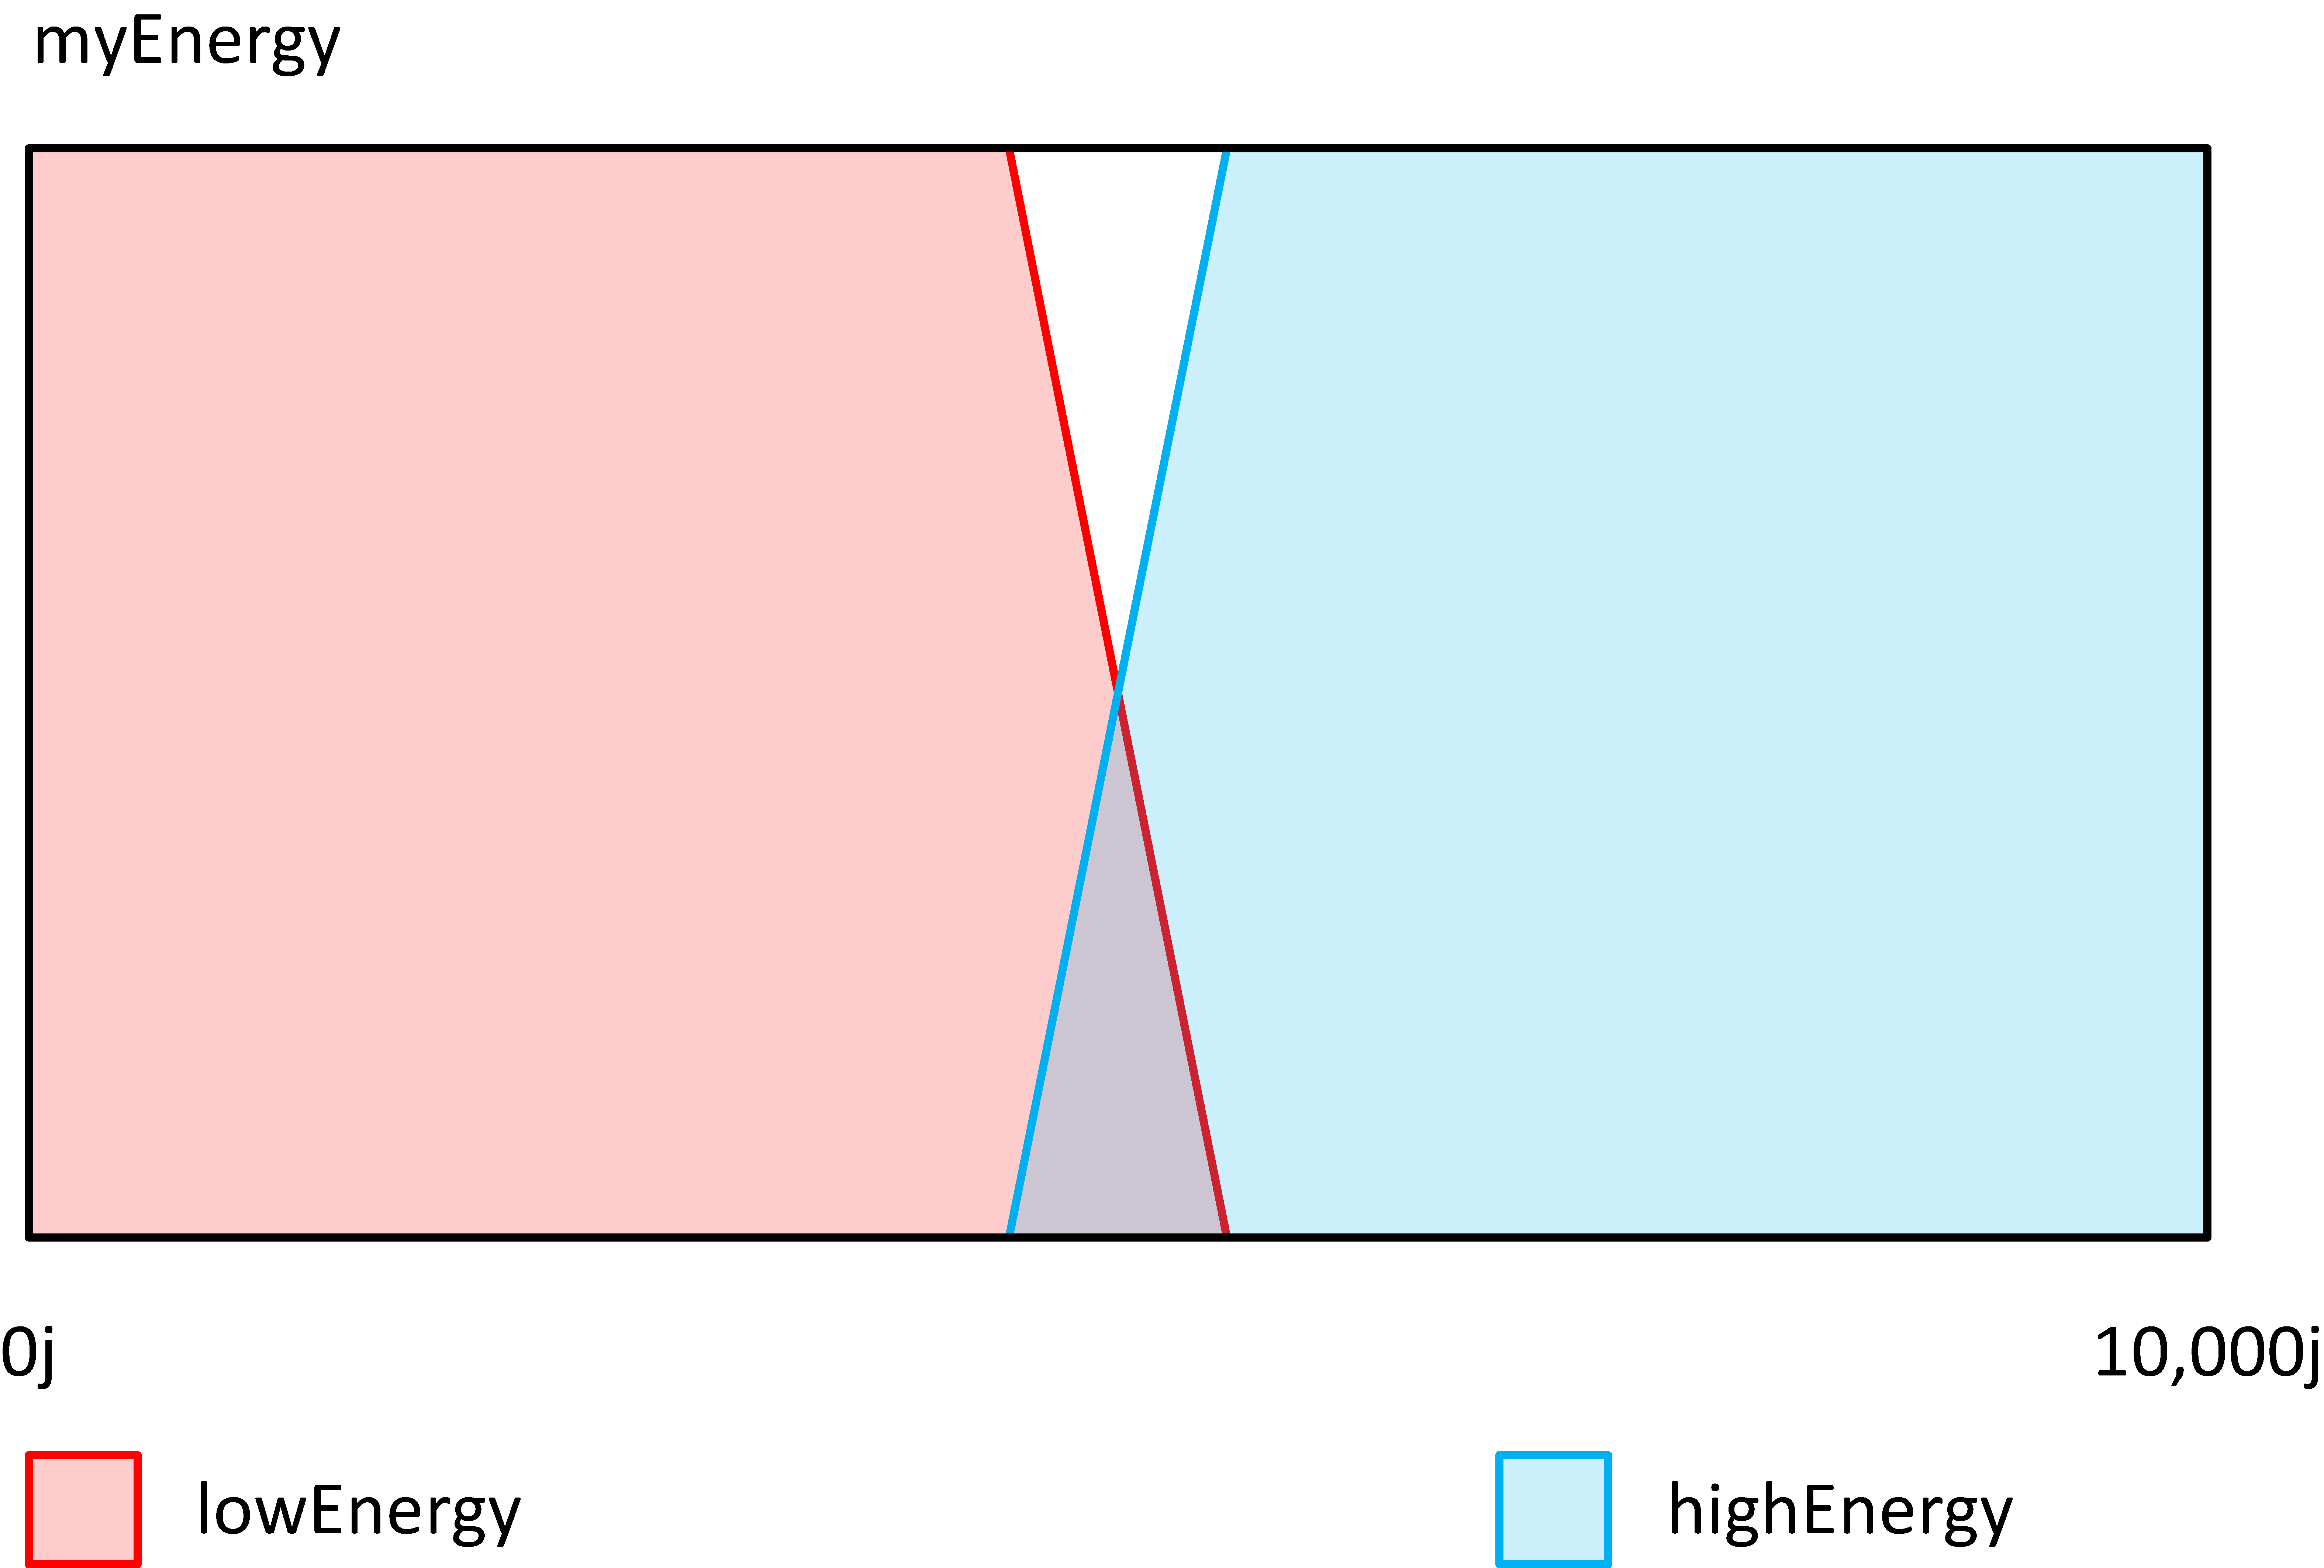
\includegraphics[scale=0.08]{./img/pdf/myEnergySets.pdf}
\end{figure}

\subsection{Target variables}

The sensor returns a list of all the enemy saucers currently in the battle space. This controller only considers the closest saucer as the target, and ignores all other saucers in the list.

\subsubsection{targetDist}

The linguistic variable \emph{targetDist} is the distance from the player to the target. The universe of disclosure for \emph{targetDist} is between 0m and 4802.3m, and the fuzzy sets are defined as \emph{close}, \emph{near}, and \emph{far}.

\begin{figure}[H]
\centering
\caption{\emph{targetDist} fuzzy sets}
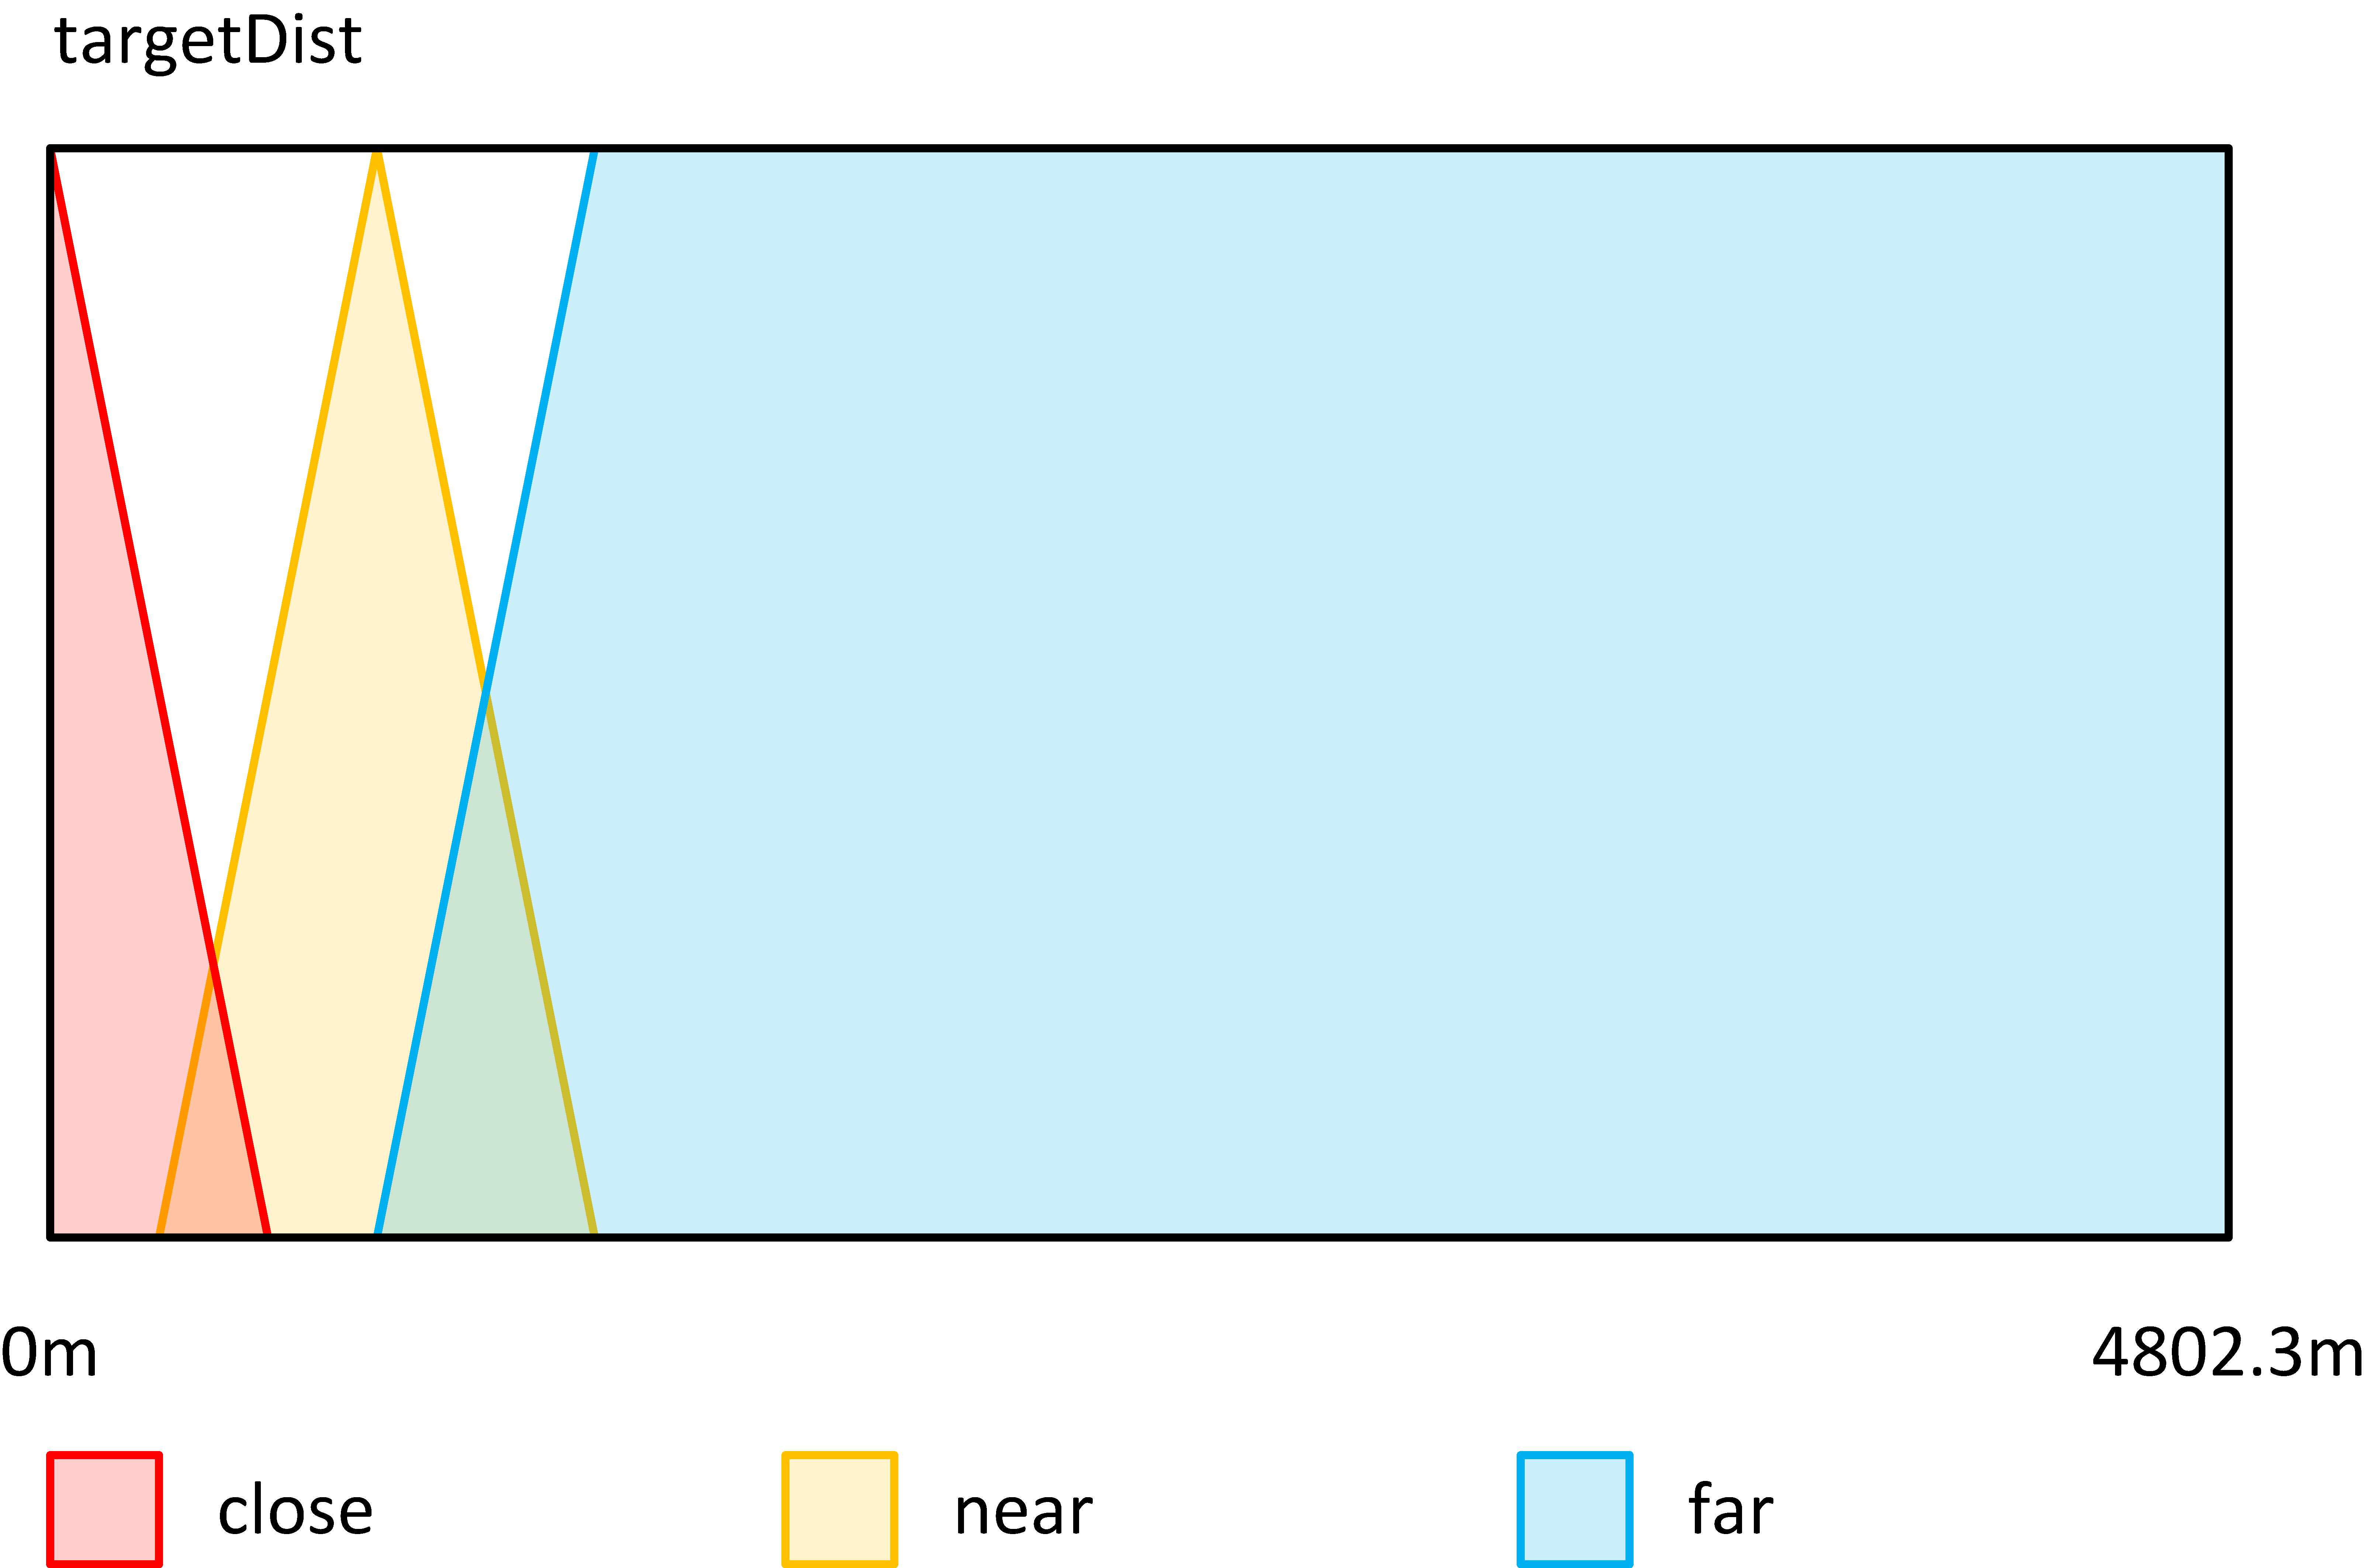
\includegraphics[scale=0.08]{./img/pdf/targetDistSets.pdf}
\end{figure}

\subsubsection{targetAspect}

The linguistic variable \emph{targetAspect} is the direction of the target in relation to the player. The universe of disclosure for \emph{targetAspect} is between -360$^{\circ}$ and +360$^{\circ}$. Positive values rotate to the left, and negative values rotate to the right. The fuzzy sets selected relate to clock positions, similar to what fighter pilots might call out in combat. There are three twelve o'clock positions due to the two revolutions between -360$^{\circ}$ and +360$^{\circ}$.

\begin{figure}[H]
\centering
\caption{\emph{targetAspect} fuzzy sets}
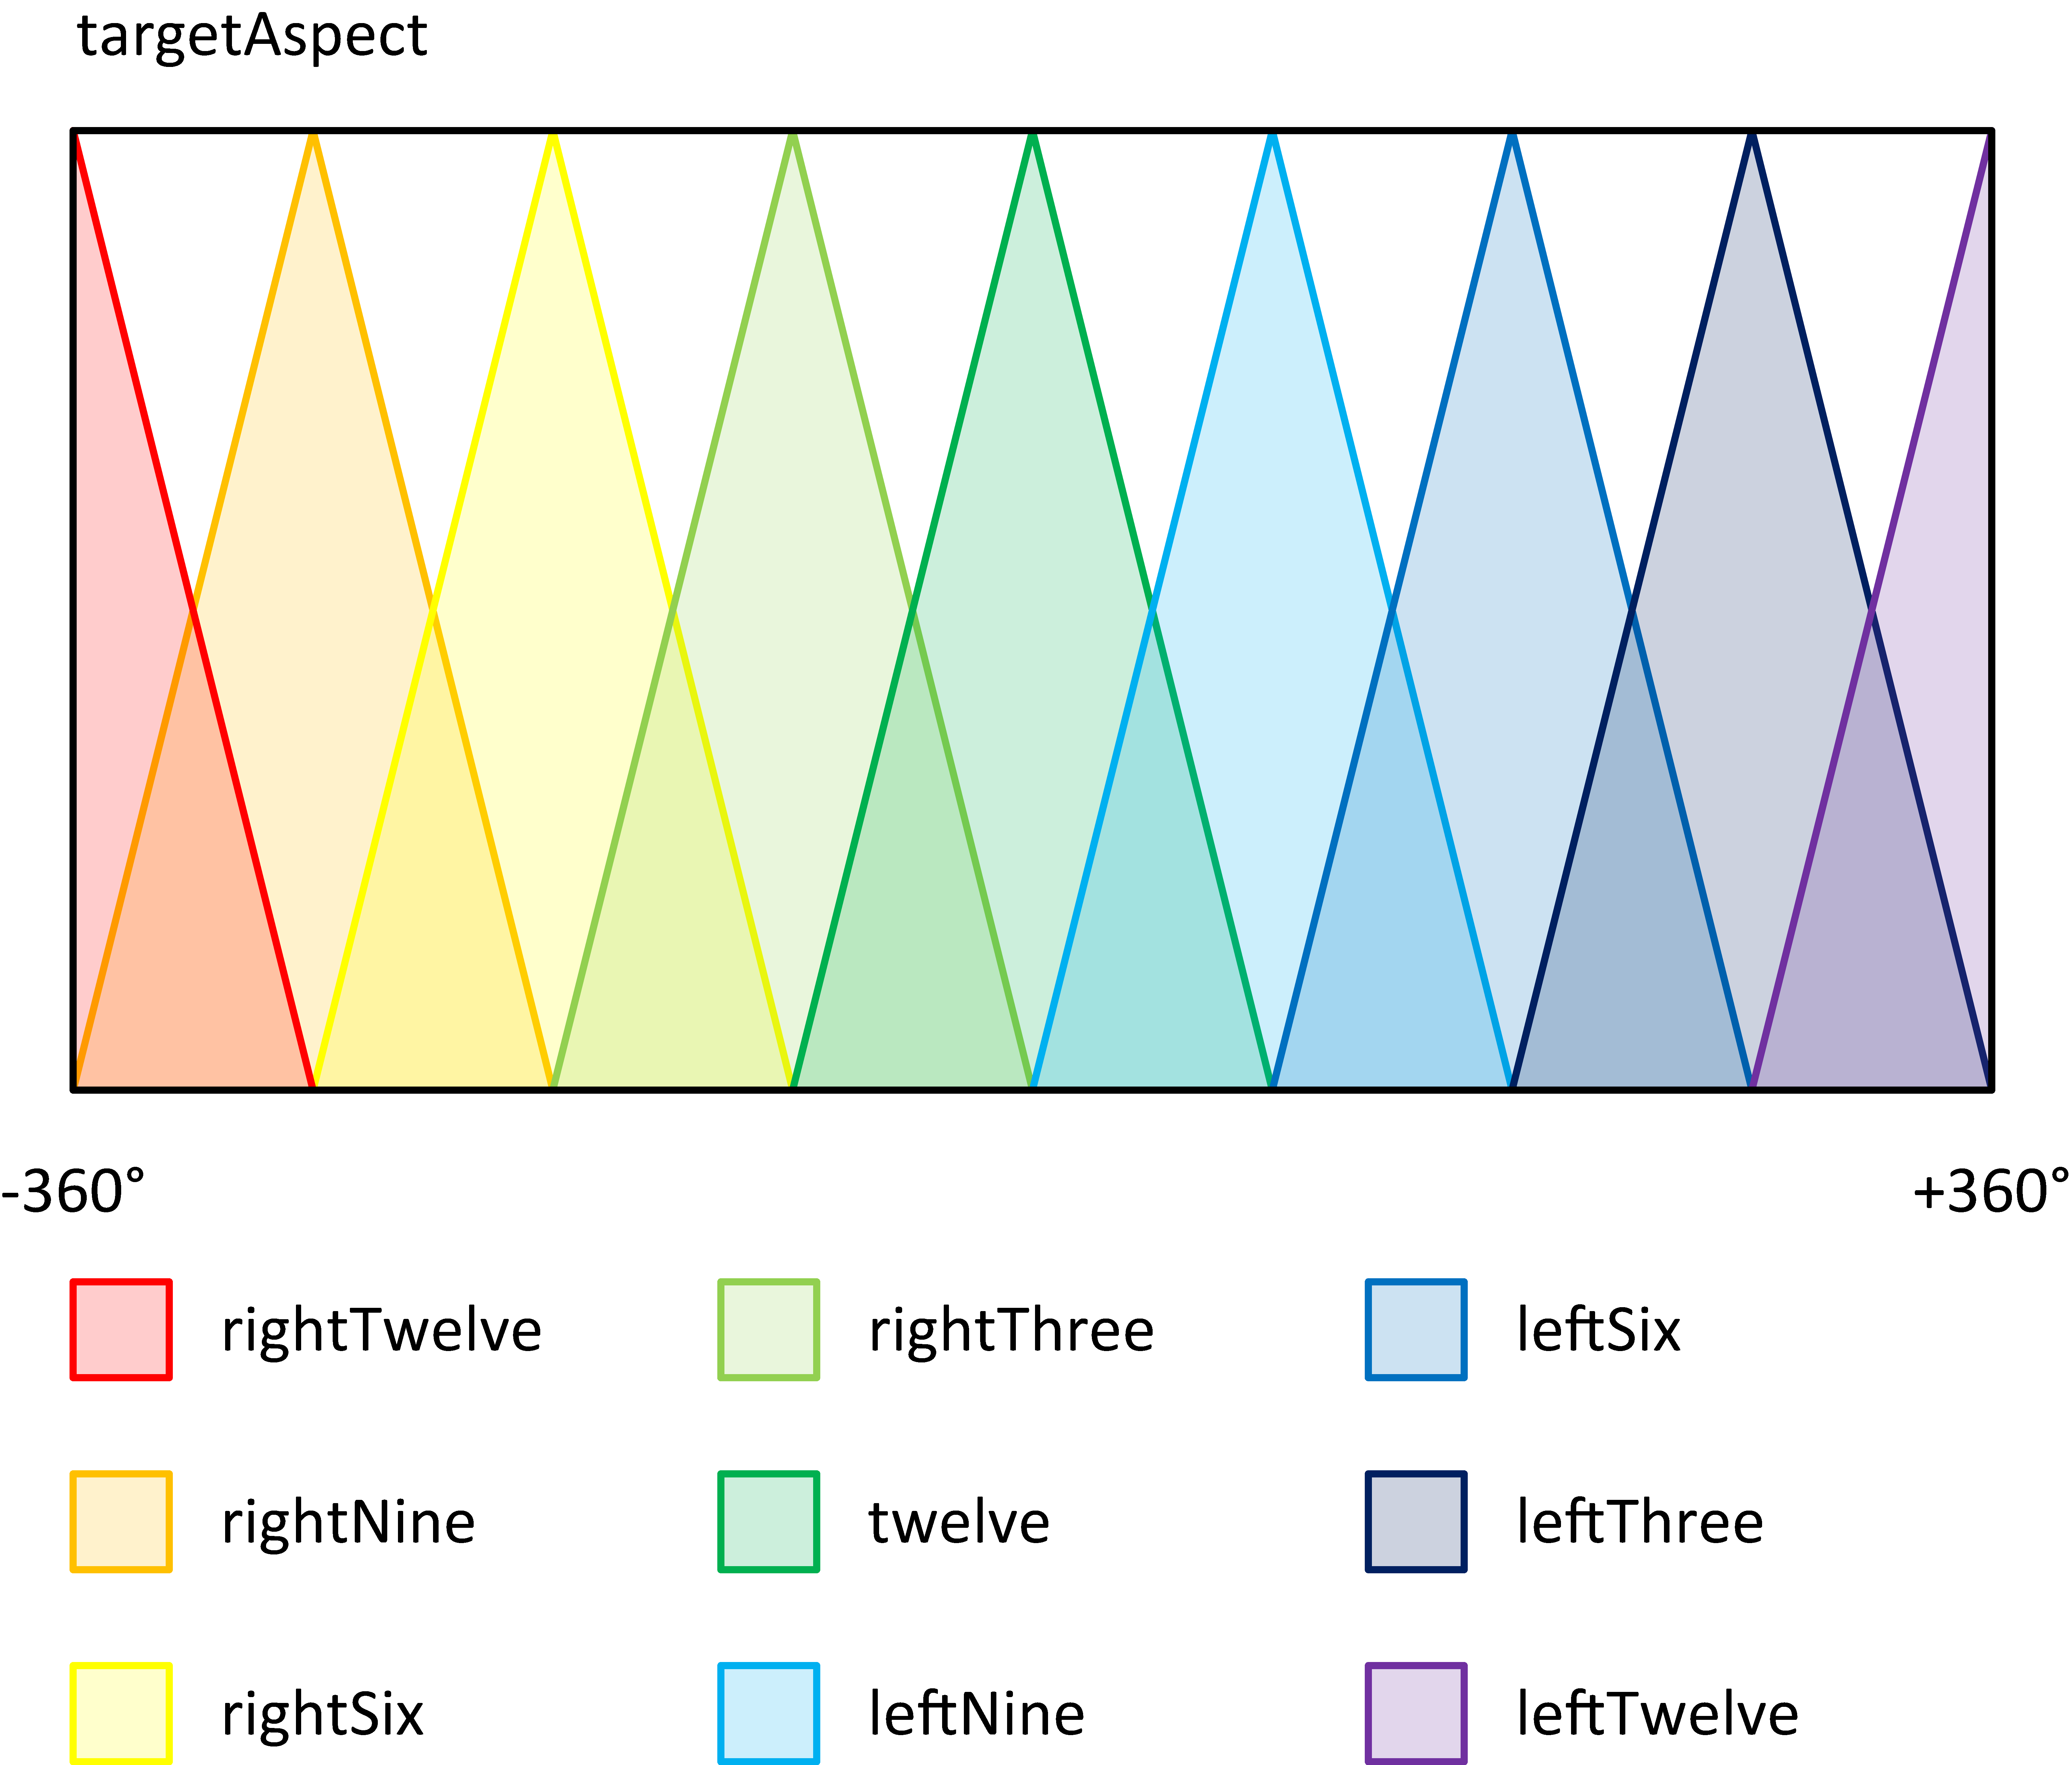
\includegraphics[scale=0.08]{./img/pdf/targetAspectSets.pdf}
\end{figure}

\subsubsection{targetAngleOff}

The linguistic variable \emph{targetAngleOff} relates to the target's current heading, in relation to the player's current heading. For example, if the target is heading towards the player perpendicularly from the right, the target's angle-off would be +90$^{\circ}$. Similarly, if the target has the exact same heading as the player, the target's angle-off would be 0$^{\circ}$. Again, positive values rotate to the left, and negative values rotate to the right. The universe of disclosure is between -360$^{\circ}$ and +360$^{\circ}$. The fuzzy sets selected mimic clock positions, similar to \emph{targetAspect}, however are named with degree values. A merge is when the player and target have opposite angle-off's, ie. 180$^{\circ}$. In this situation, if the player and target were in front of each other, they would facing each other, and would be about to directly pass each other, in a ``merge''.

\begin{figure}[H]
\centering
\caption{\emph{targetAngleOff} fuzzy sets}
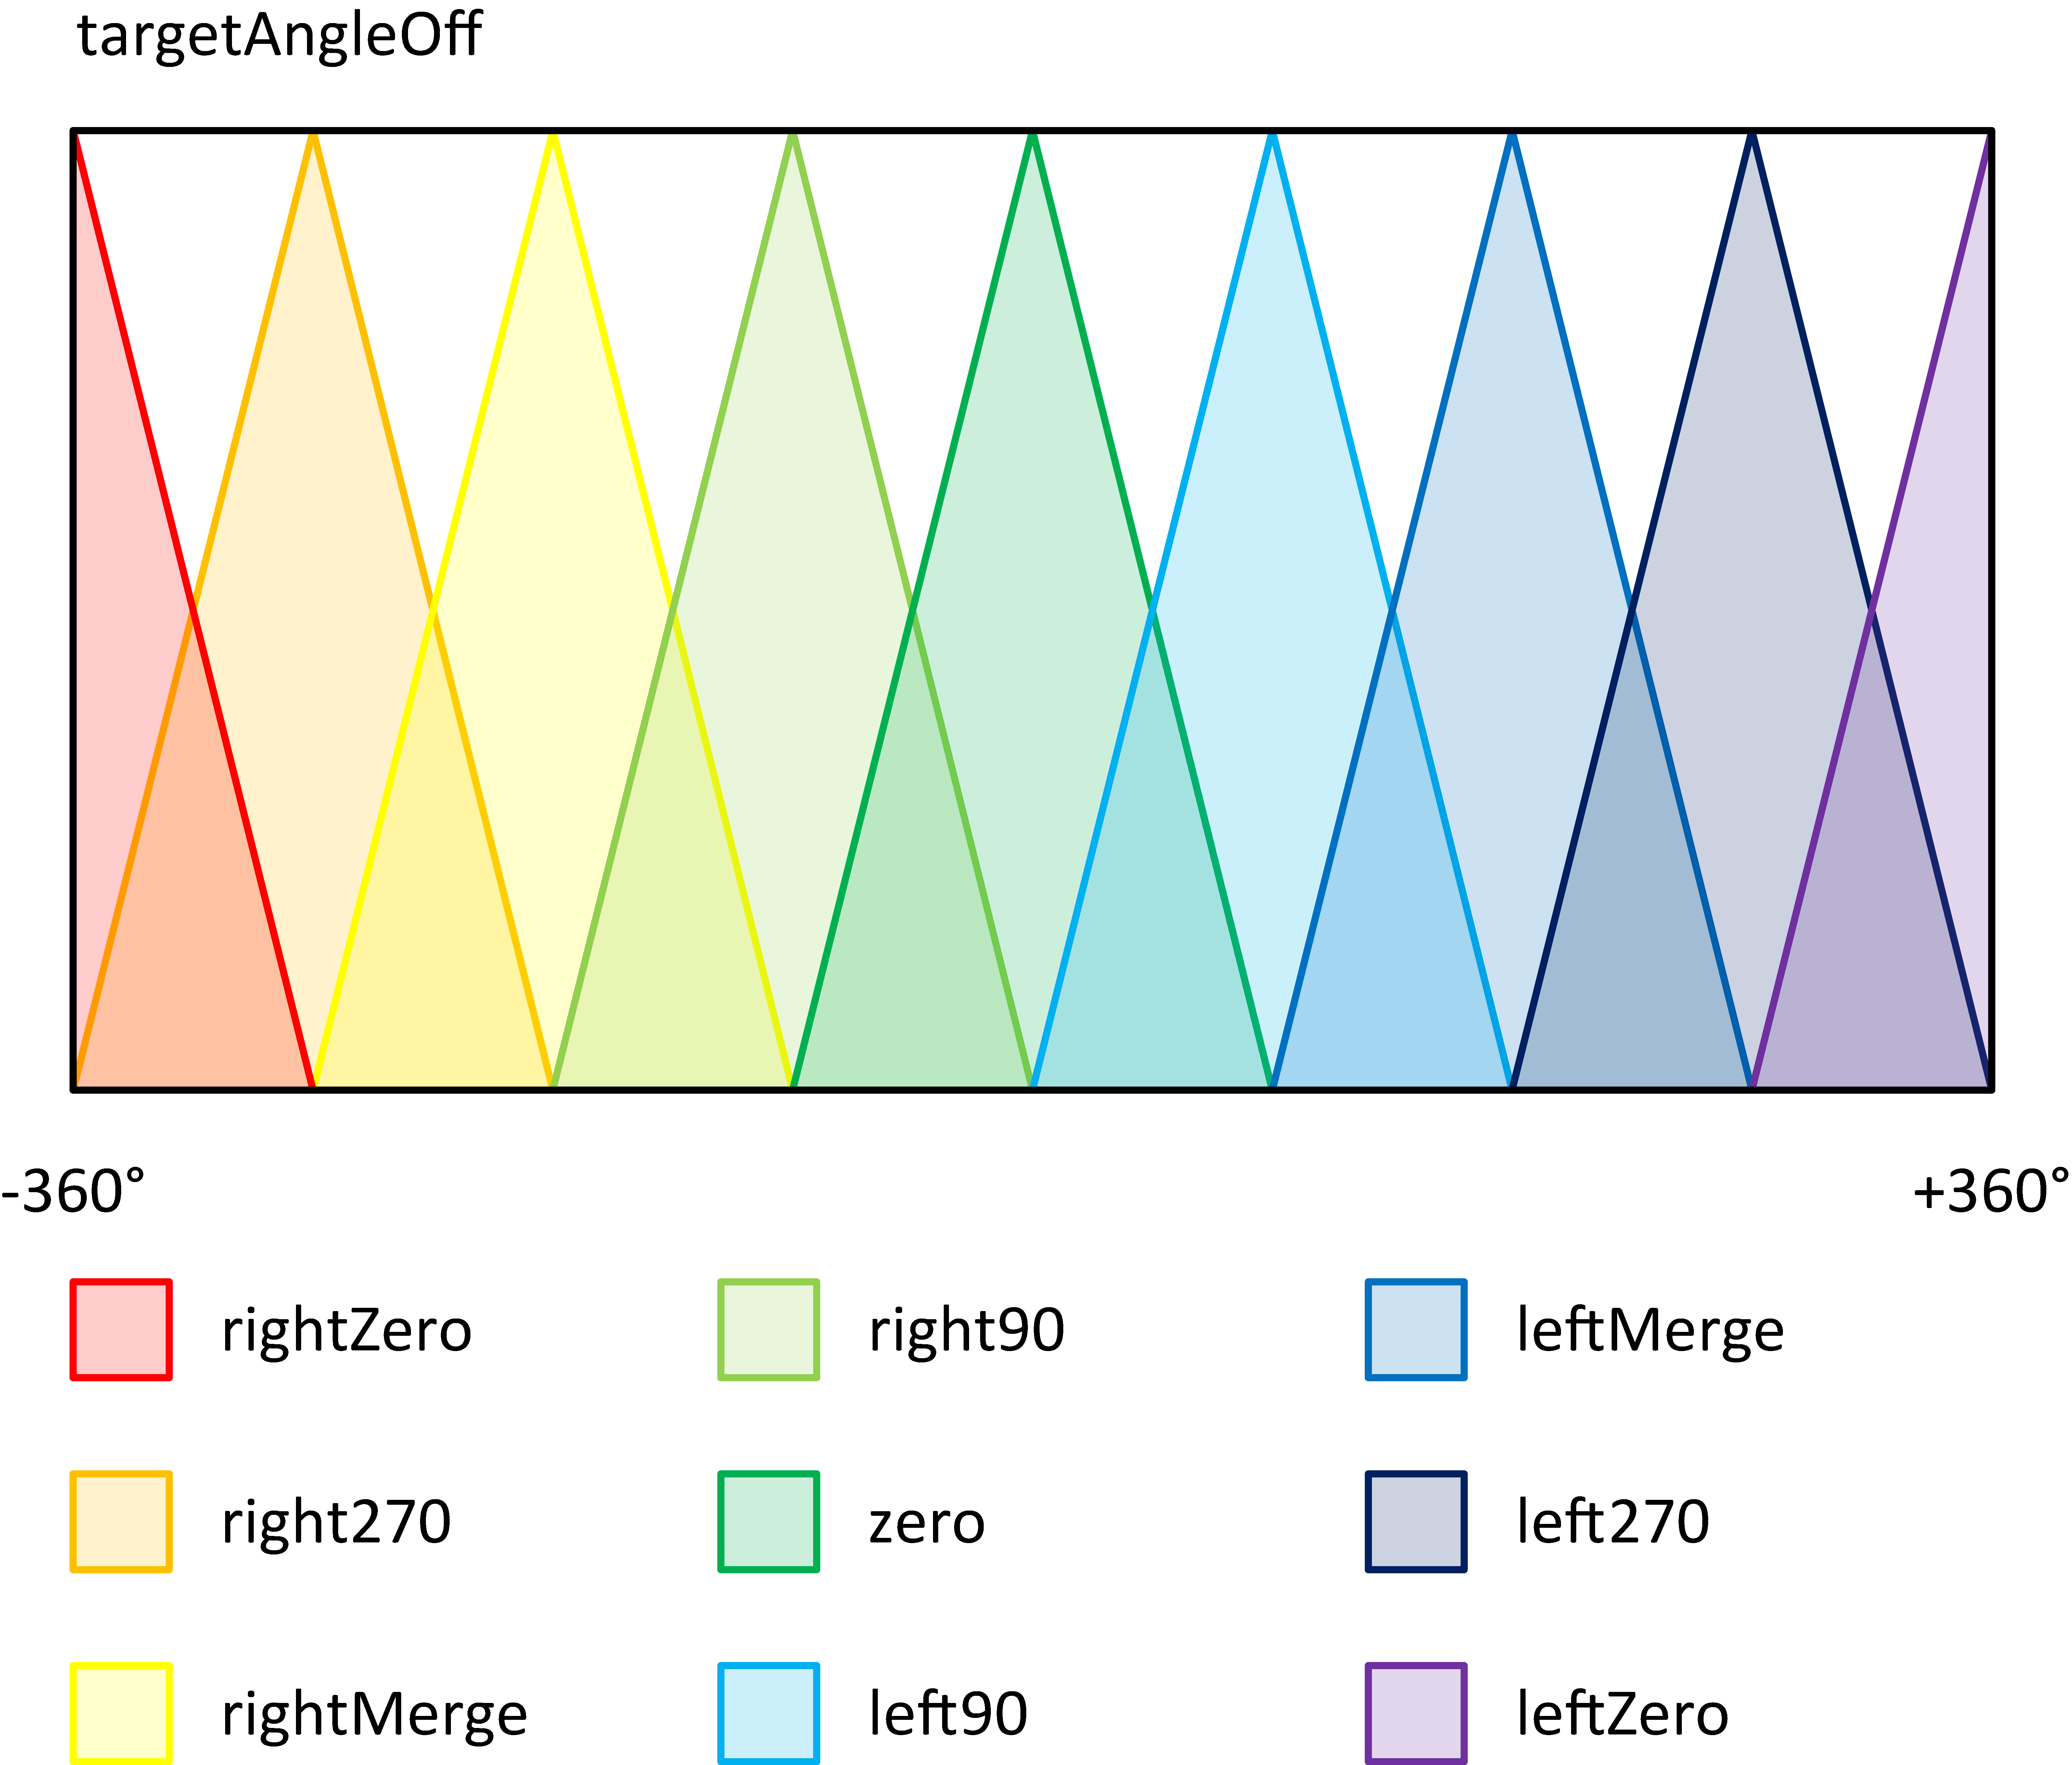
\includegraphics[scale=0.08]{./img/pdf/targetAngleOffSets.pdf}
\end{figure}

\subsubsection{targetEnergyDiff}

The linguistic variable \emph{targetEnergyDiff} relates to the difference between the player's energy and the current target's energy. The universe of disclosure for \emph{targetEnergyDiff} is between -10,000j and +10,000j. The fuzzy sets selected for this linguistic variable are \emph{losing} and \emph{winning}.

\begin{figure}[H]
\centering
\caption{\emph{targetEnergyDiff} fuzzy sets}
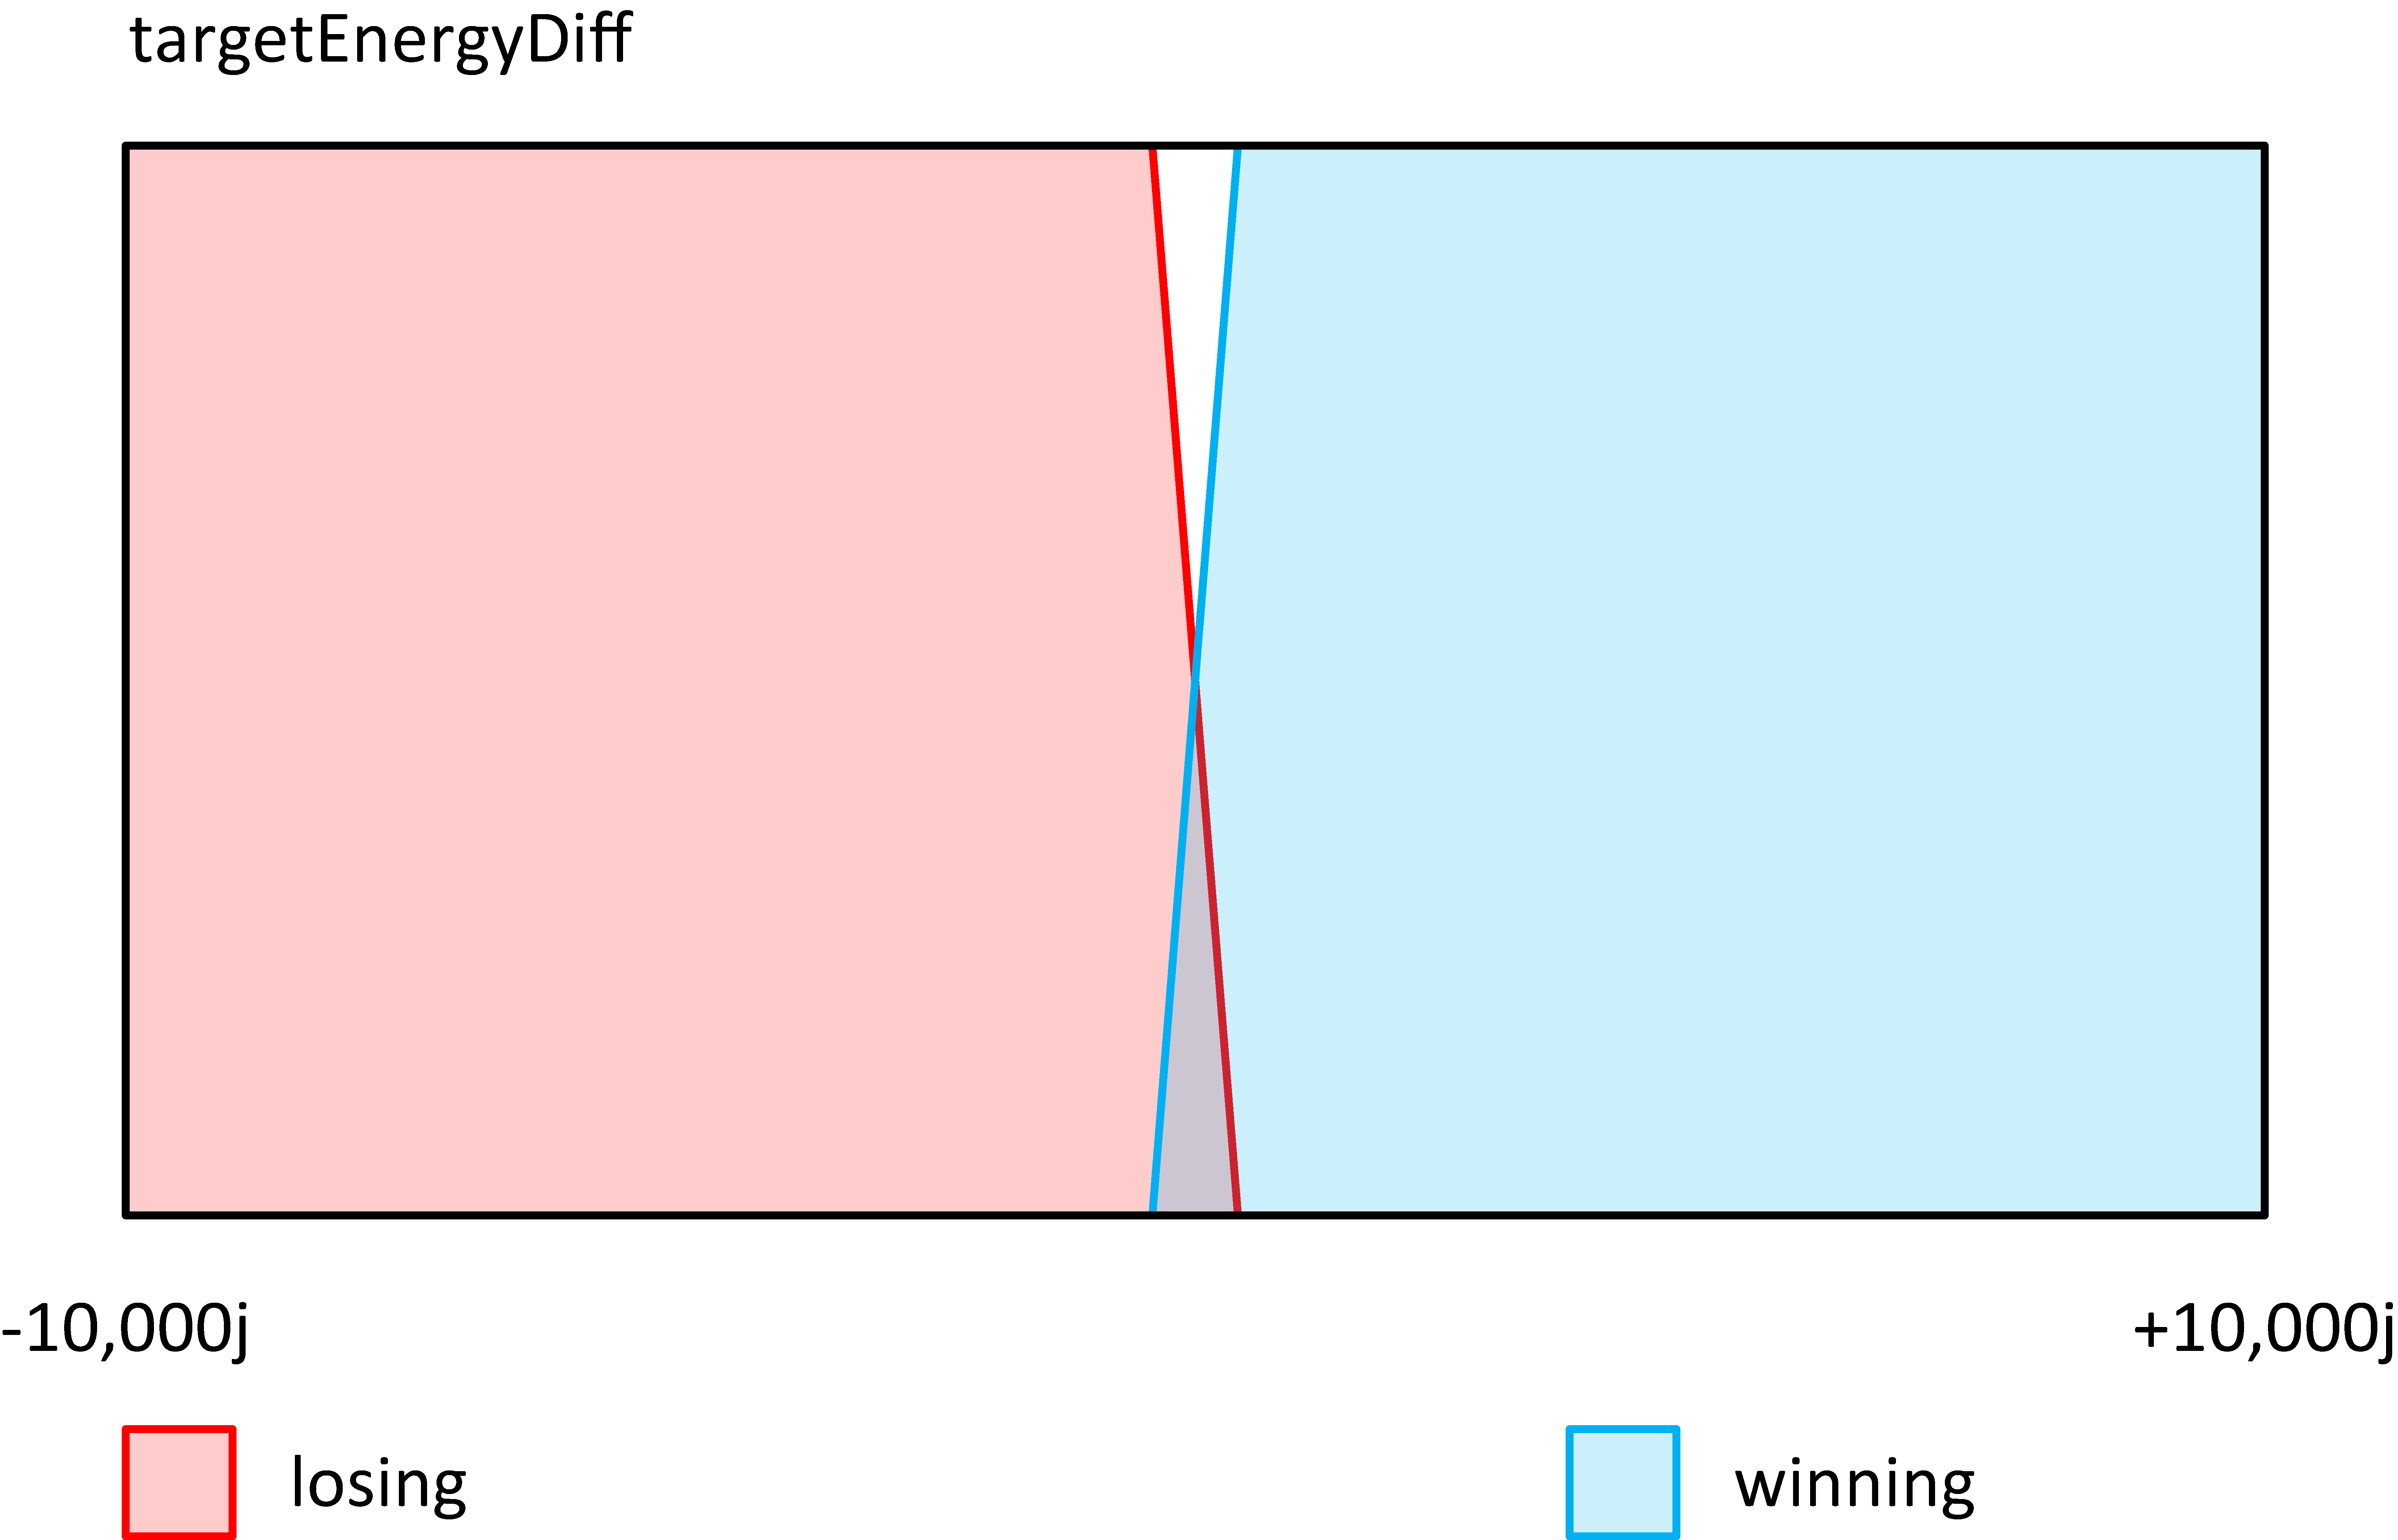
\includegraphics[scale=0.08]{./img/pdf/targetEnergyDiffSets.pdf}
\end{figure}

\subsection{Blast variables}

The sensor returns a list of all energy blasts currently in the battle space. This controller only considers the closest energy blast to dodge, and ignores all other blasts in the list.

\subsubsection{blastDist}

The linguistic variable \emph{blastDist} is the distance from the player to the energy blast. The universe of disclosure for \emph{blastDist} is between 0m and 4802.3m, and the fuzzy sets are defined as \emph{close} and \emph{far}.

\begin{figure}[H]
\centering
\caption{\emph{blastDist} fuzzy sets}
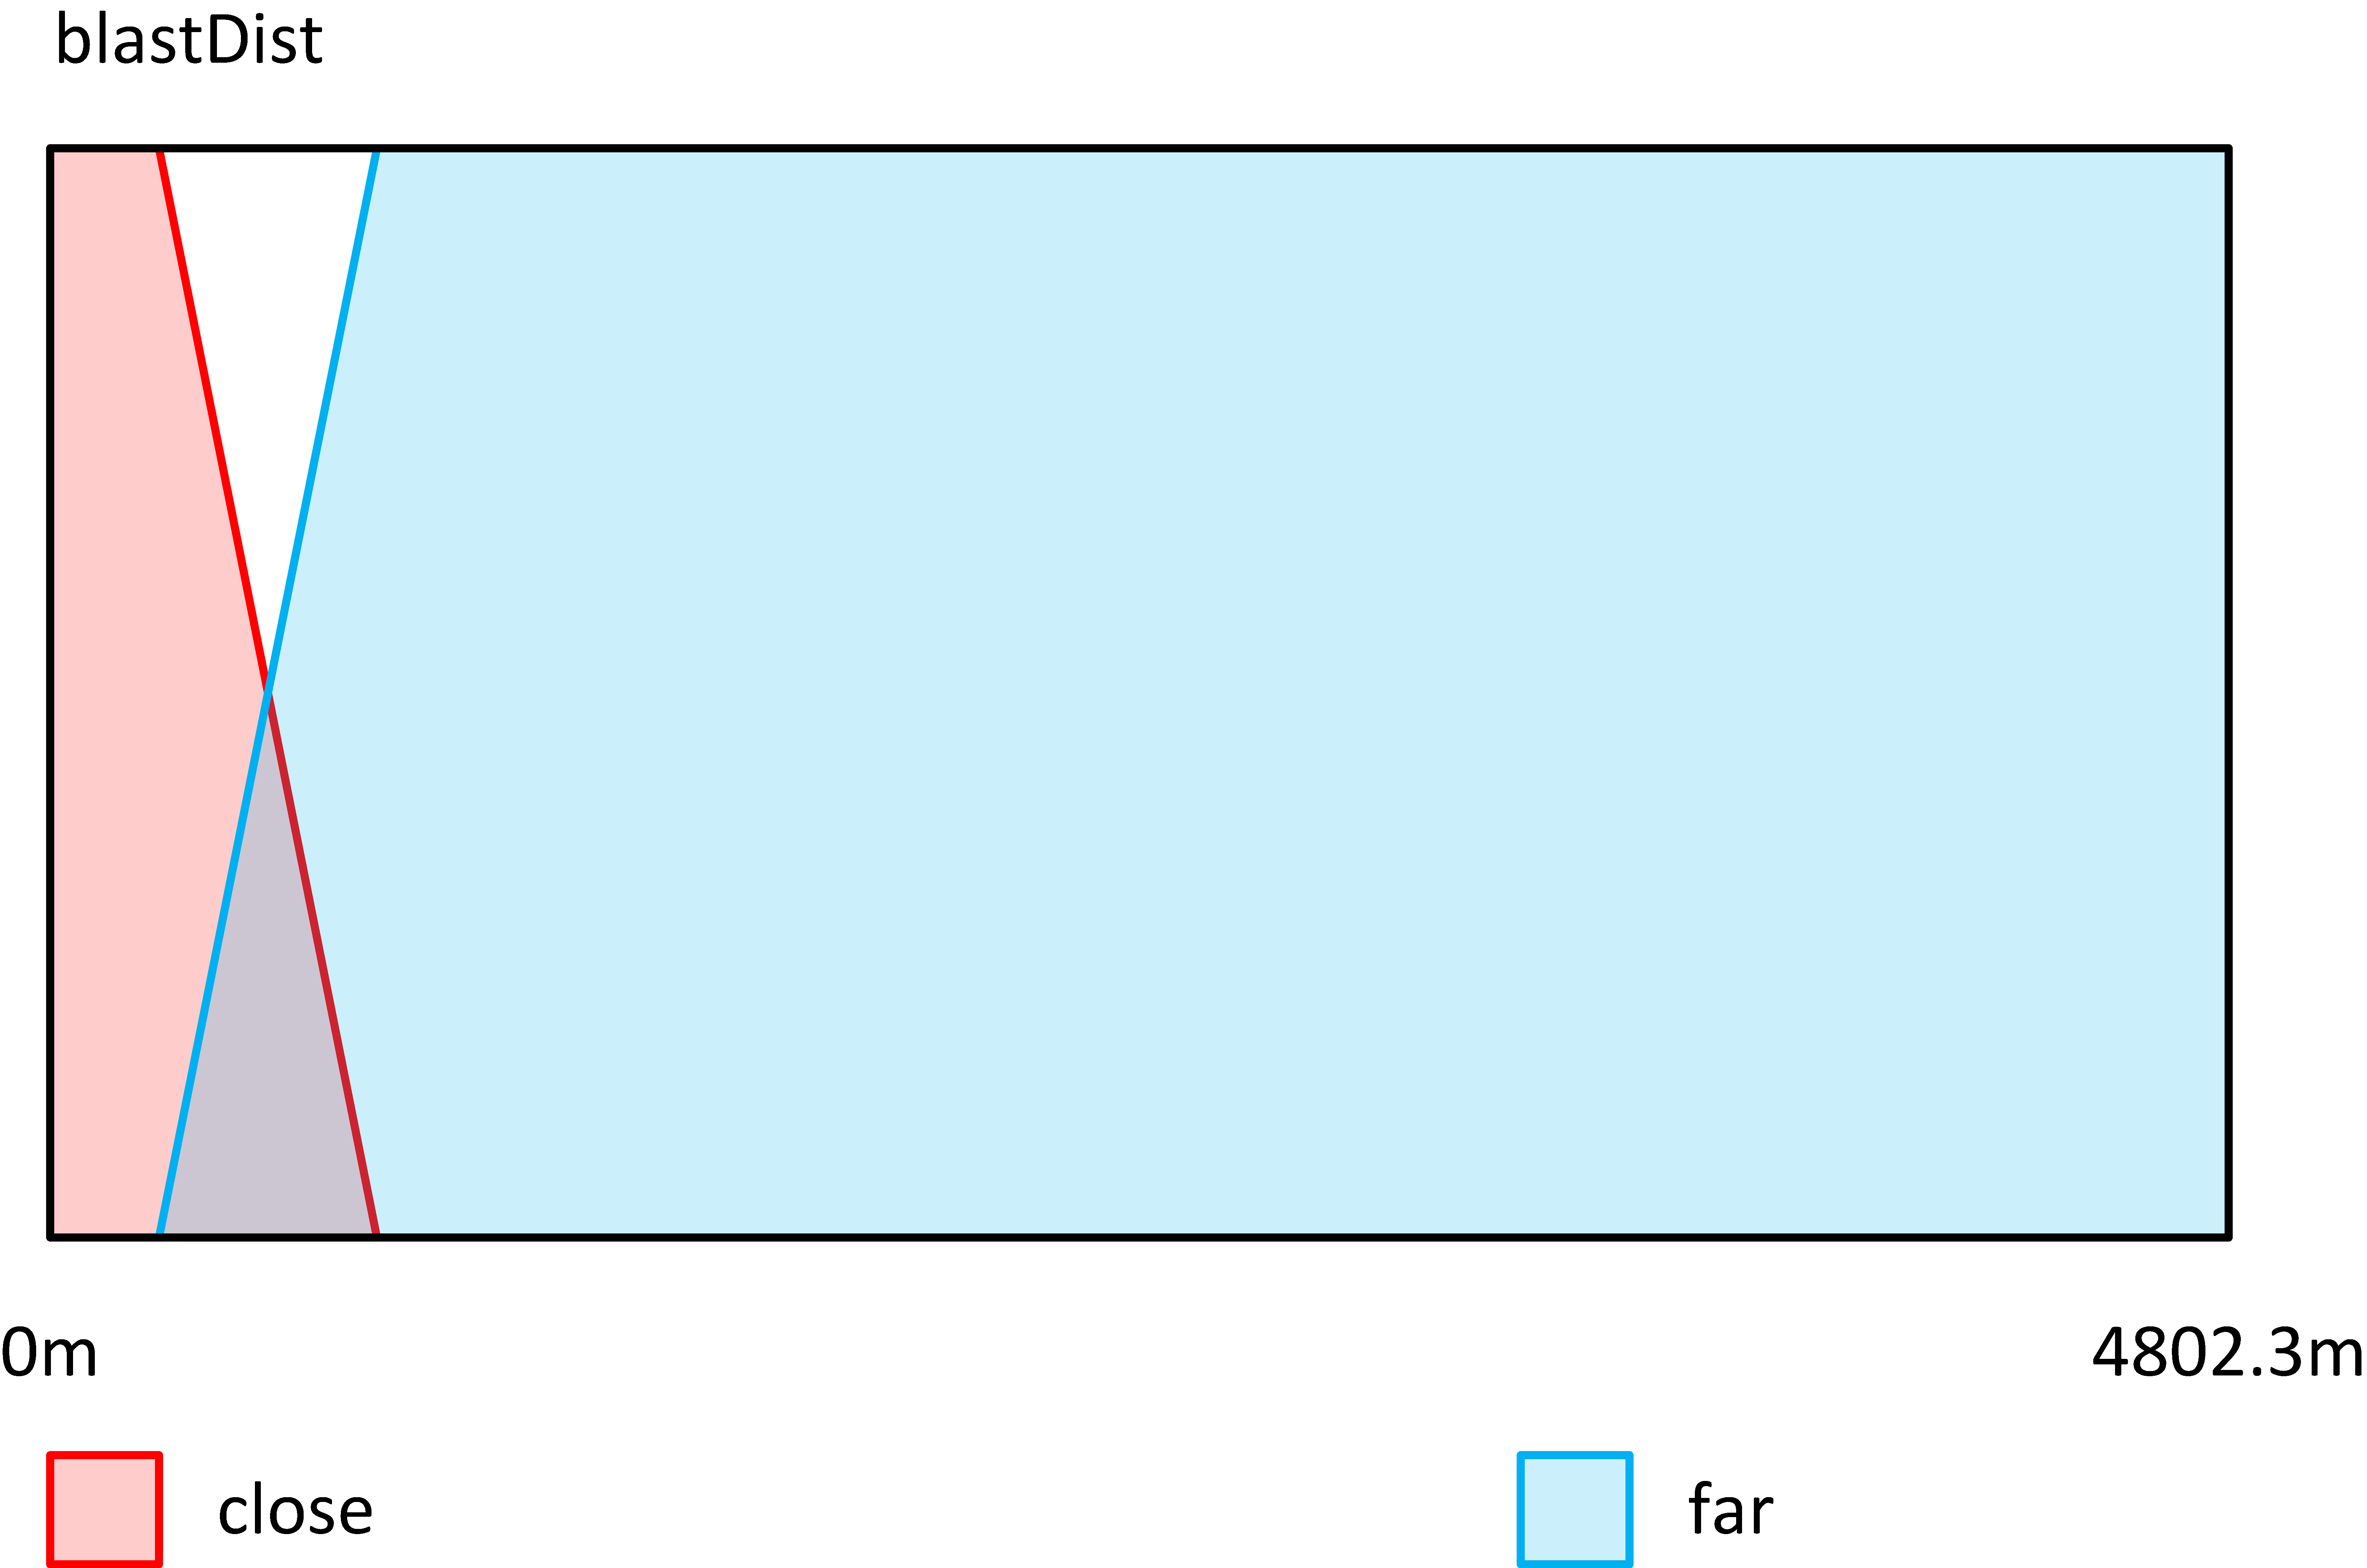
\includegraphics[scale=0.08]{./img/pdf/blastDistSets.pdf}
\end{figure}

\subsubsection{blastAspect}

The linguistic variable \emph{blastAspect} is similar to \emph{targetAspect}, but relates to the direction from the player to the energy blast. Similar fuzzy sets, based on the clock analogy have been used.

\begin{figure}[H]
\centering
\caption{\emph{blastAspect} fuzzy sets}
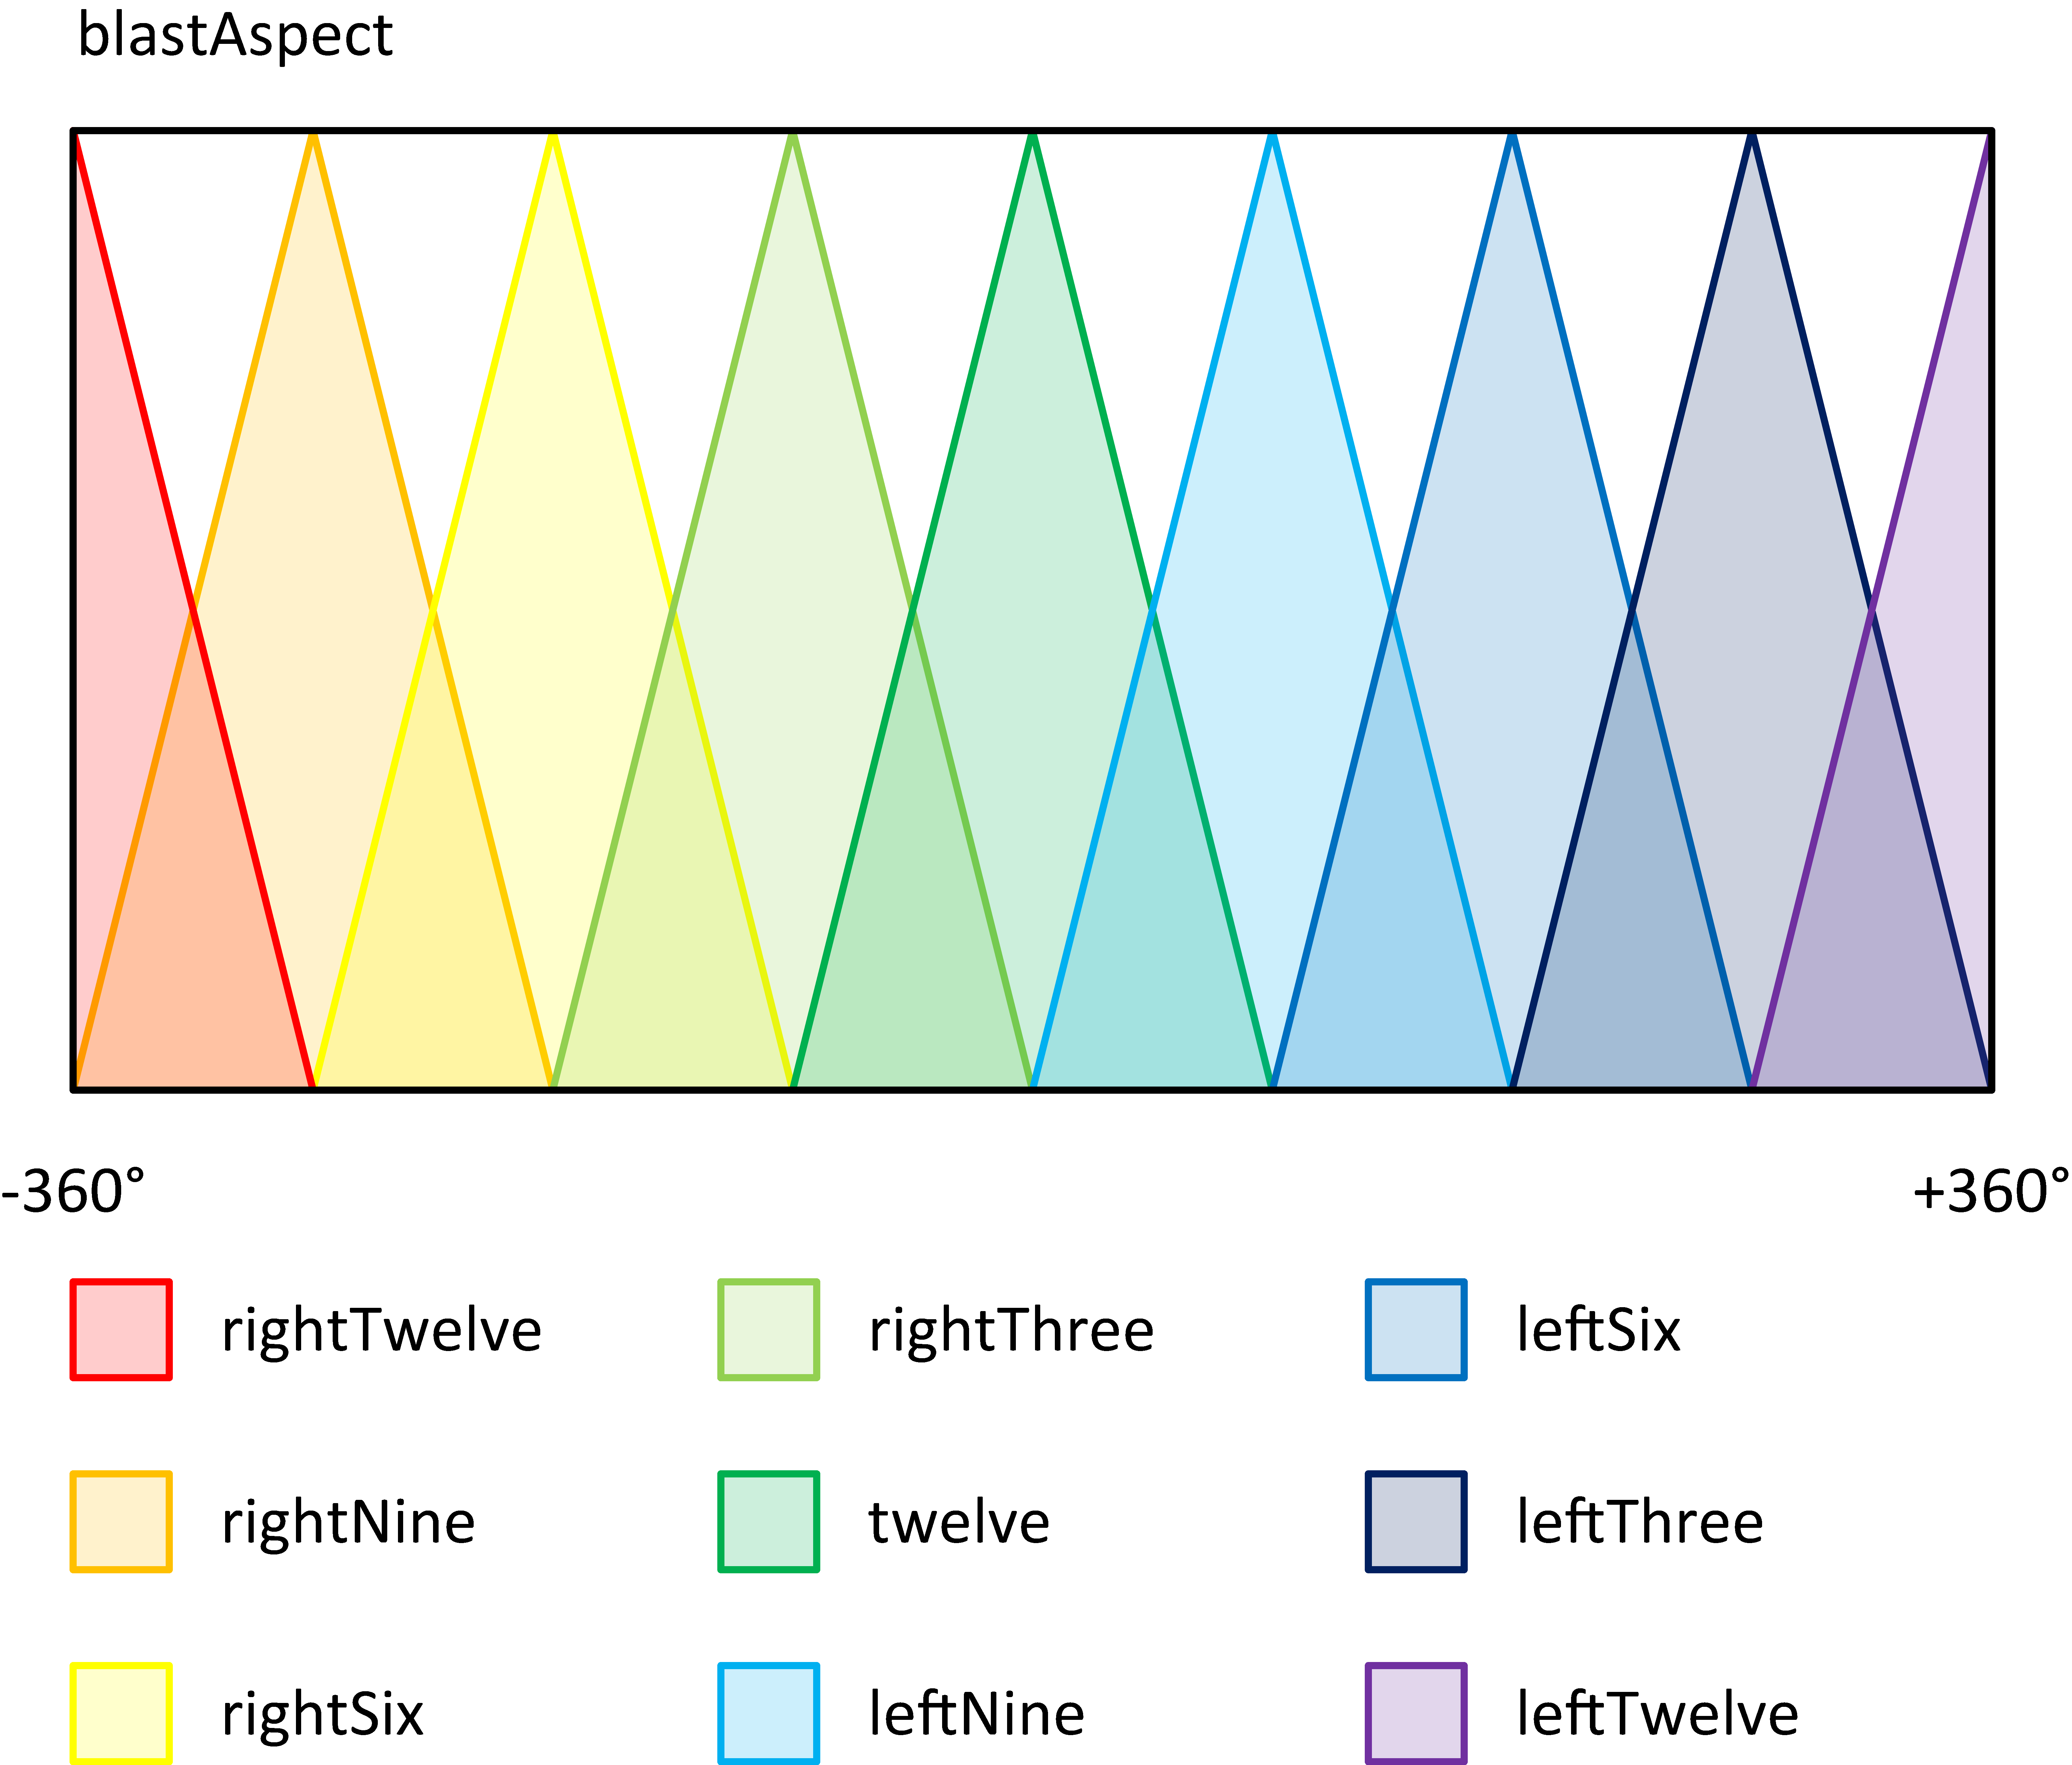
\includegraphics[scale=0.08]{./img/pdf/blastAspectSets.pdf}
\end{figure}

\subsubsection{blastAngleOff}

The linguistic variable \emph{blastAngleOff} is similar to \emph{targetAngleOff}, but references the current heading of the energy blast in relation to the player's heading. Similar fuzzy sets have also been used.

\begin{figure}[H]
\centering
\caption{\emph{blastAngleOff} fuzzy sets}
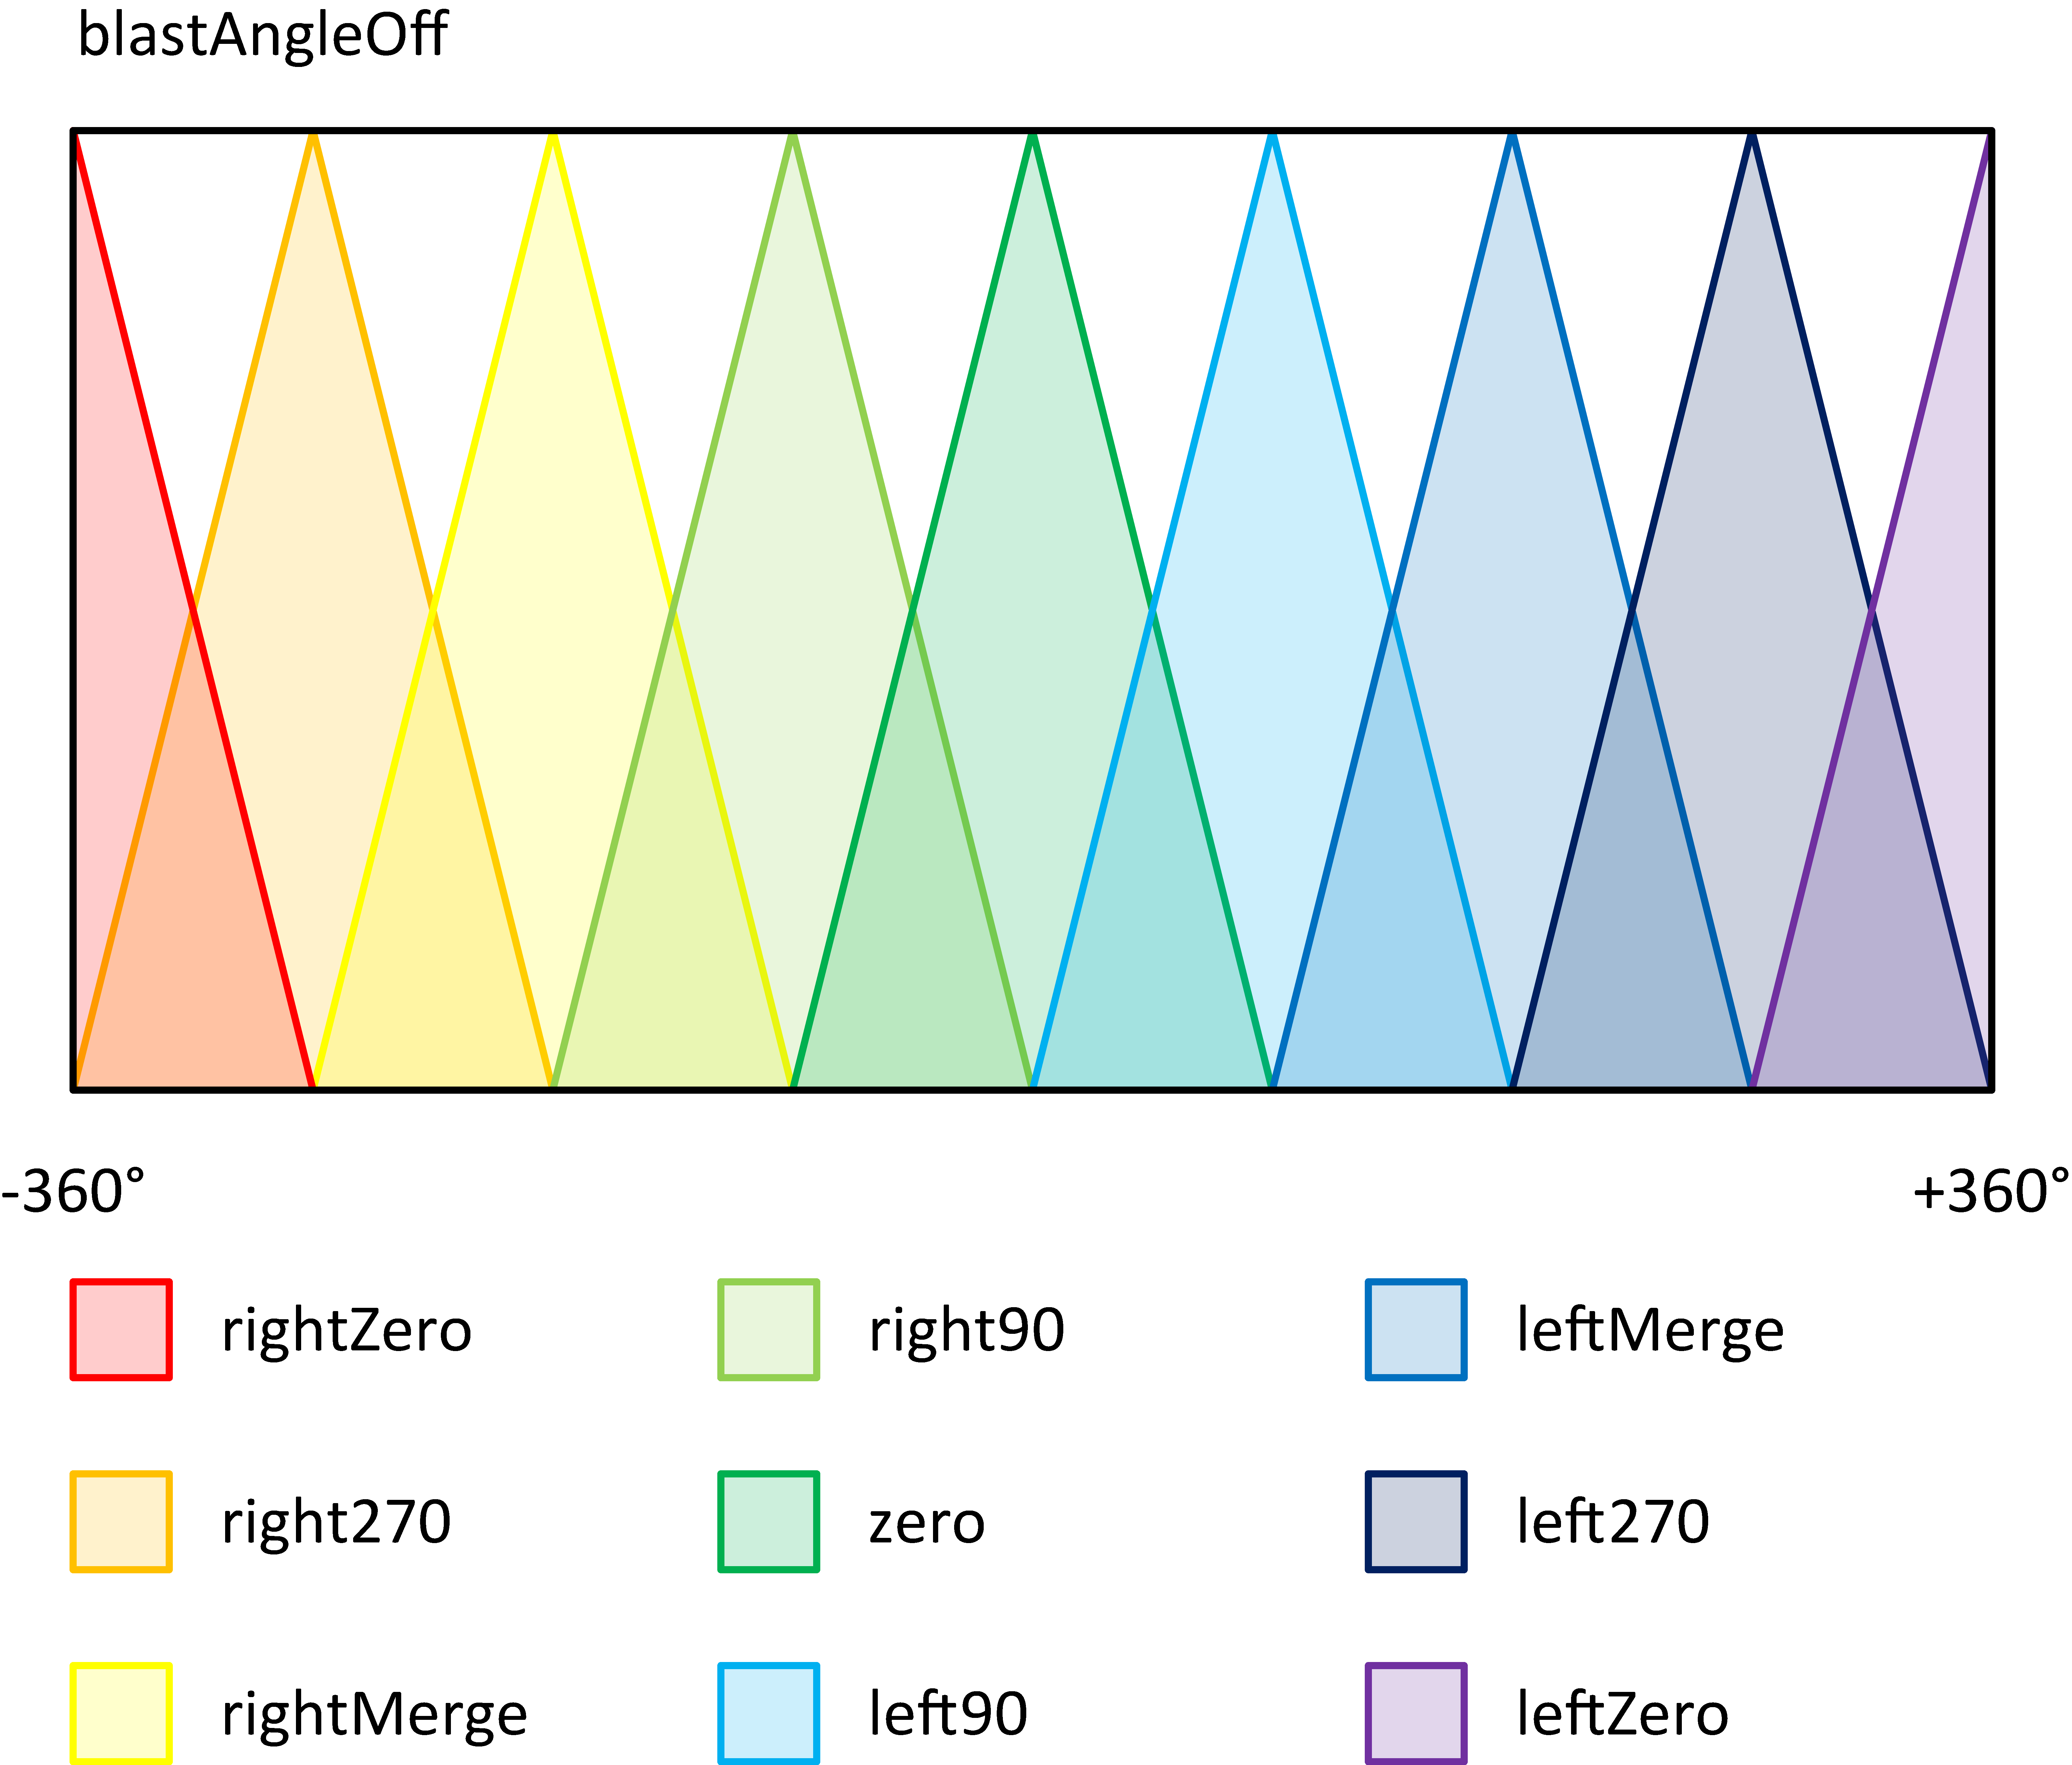
\includegraphics[scale=0.08]{./img/pdf/blastAngleOffSets.pdf}
\end{figure}

\subsection{Powerup variables}

The sensor returns a list of all powerups that currently exist in the battle space. To conserve energy, this controller only reacts to powerups only if they are nearby, and assumes that powerups that are far would most likely be consumed by an enemy by the time the player arrives.

\subsubsection{powerUpDist}

The linguistic variable \emph{powerUpDist} is the distance between the target and the powerup. Similar to \emph{targetDist}, the universe of disclosure is between 0m and 4802.3m. Similar fuzzy sets have also been used.

\begin{figure}[H]
\centering
\caption{\emph{powerUpDist} fuzzy sets}
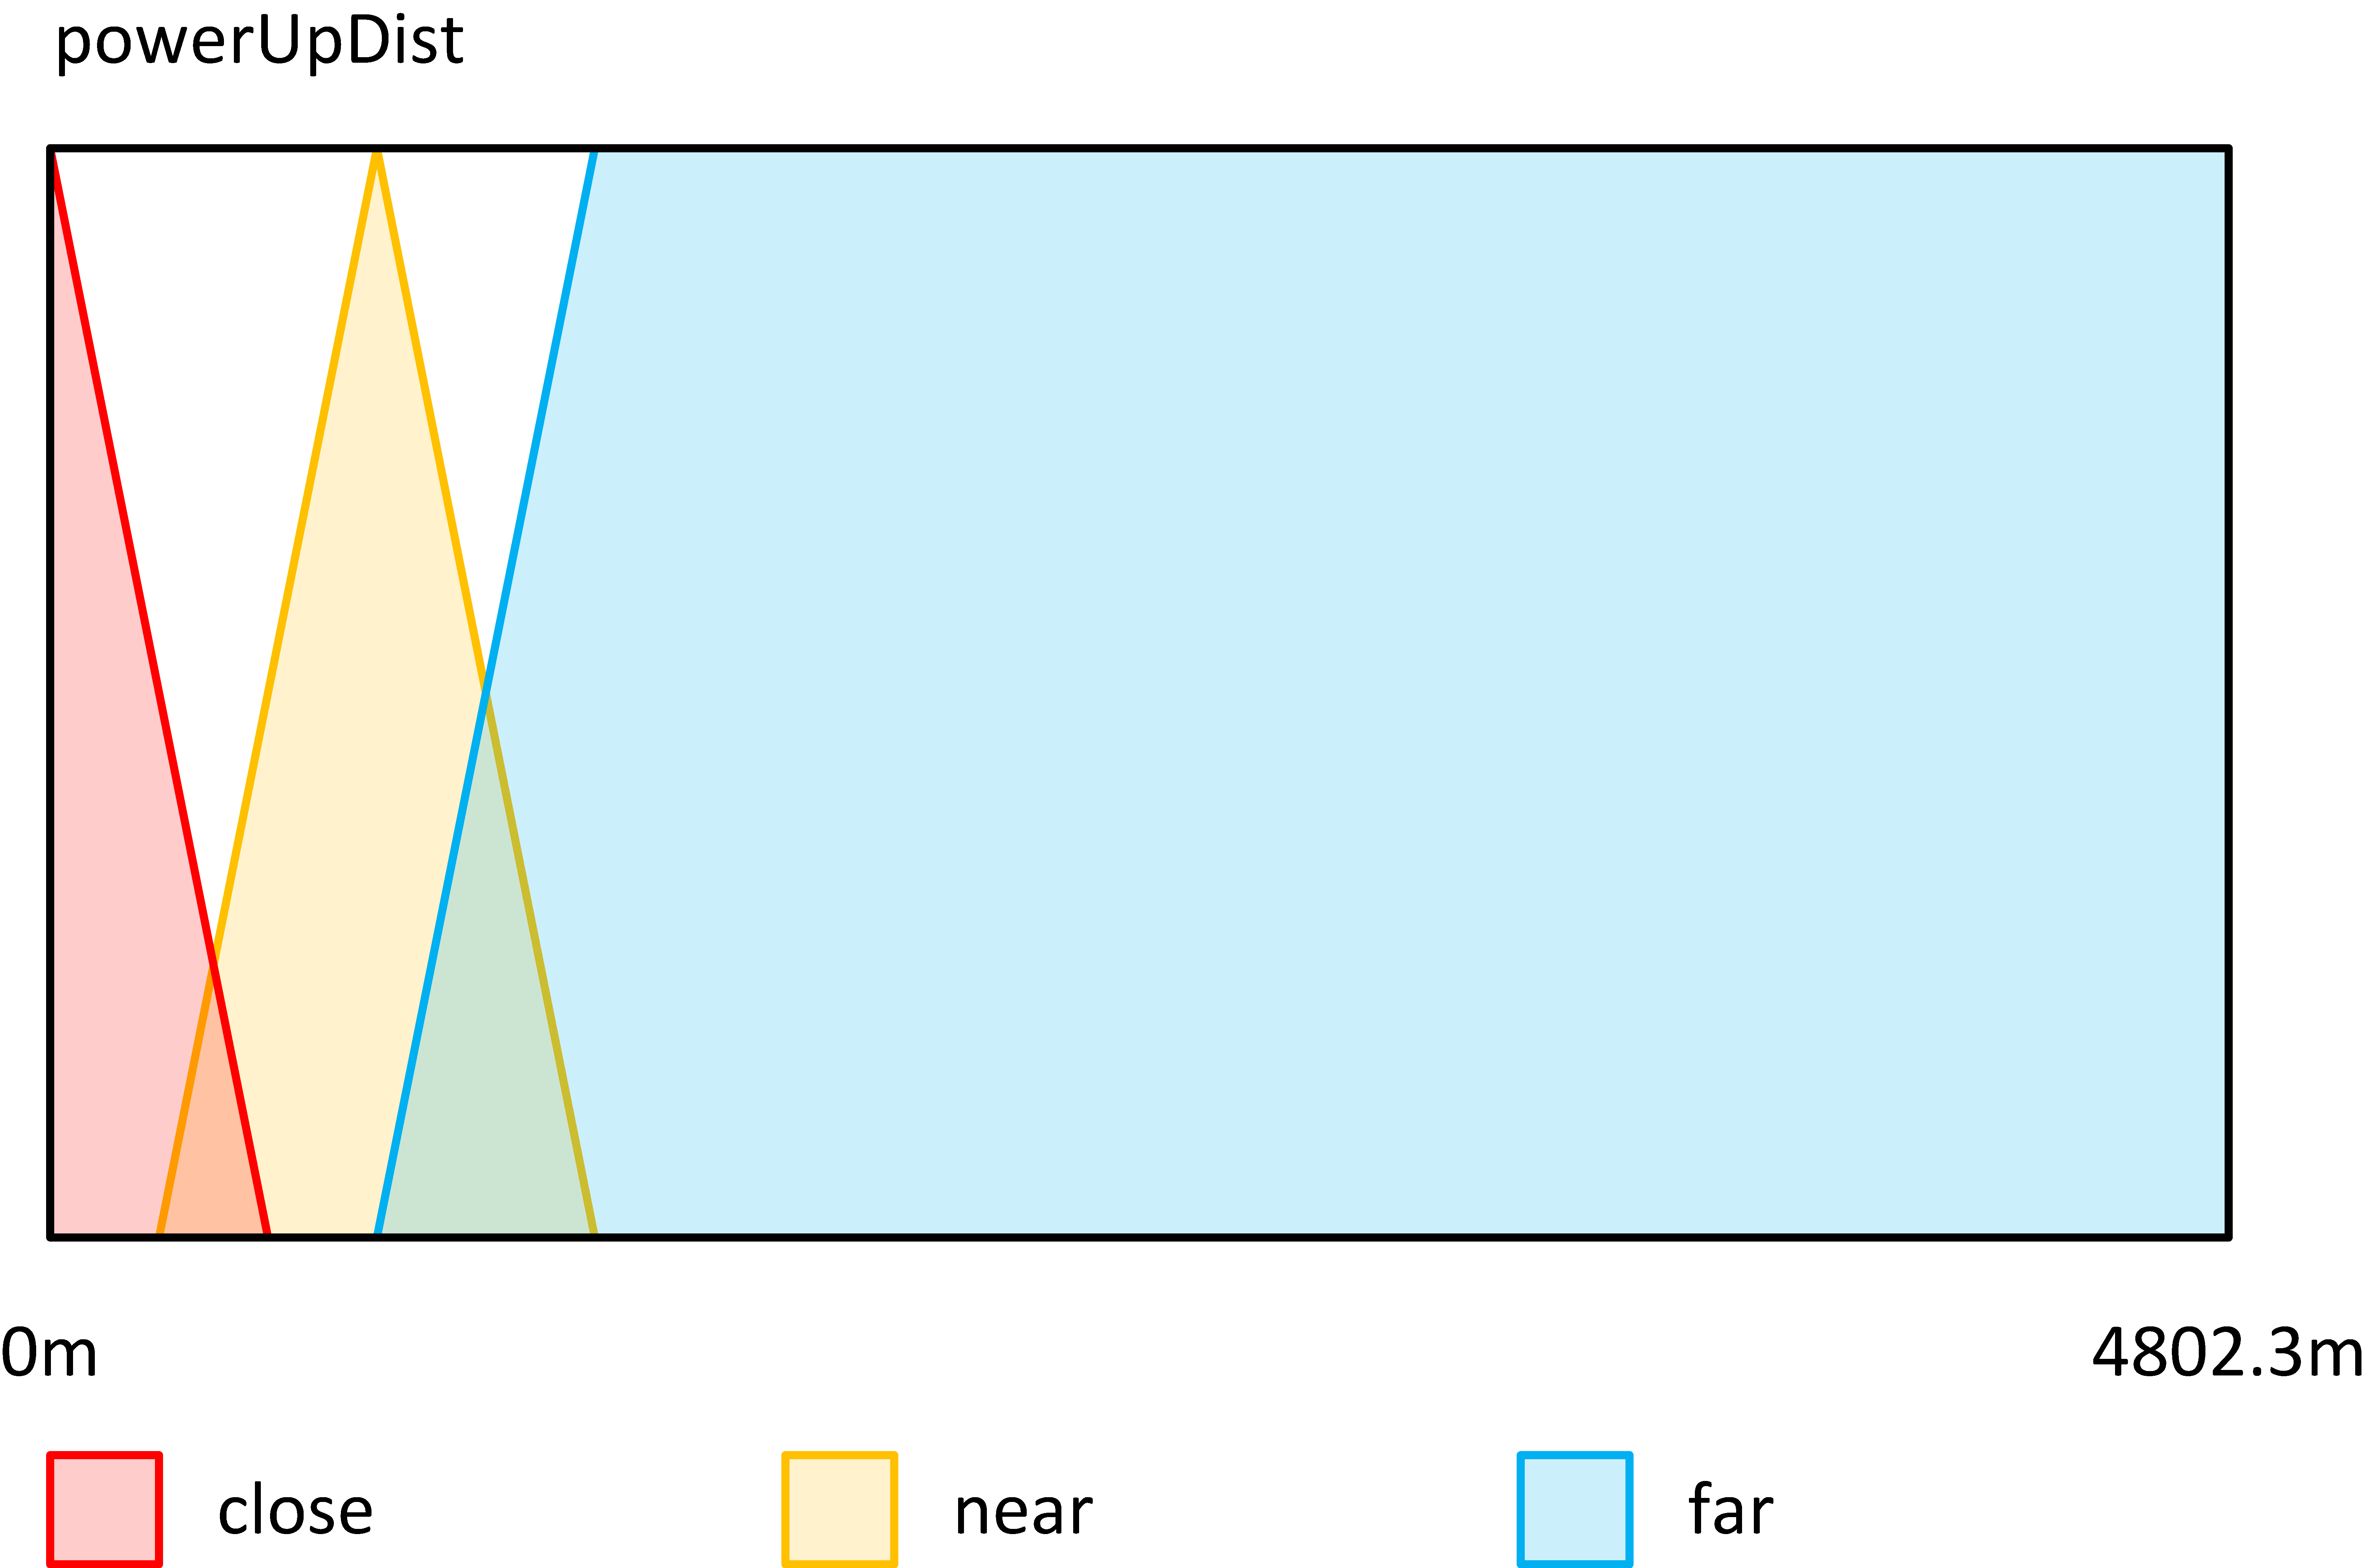
\includegraphics[scale=0.08]{./img/pdf/powerUpDistSets.pdf}
\end{figure}

\subsubsection{powerUpAspect}

The linguistic variable \emph{powerUpAspect} is the direction of the powerup in relation to the player. Again, the clock analogy has been used to determine the fuzzy sets. However, the angle-off of the powerup is not considered, since it is stationary and does not change its heading.

\begin{figure}[H]
\centering
\caption{\emph{powerUpAspect} fuzzy sets}
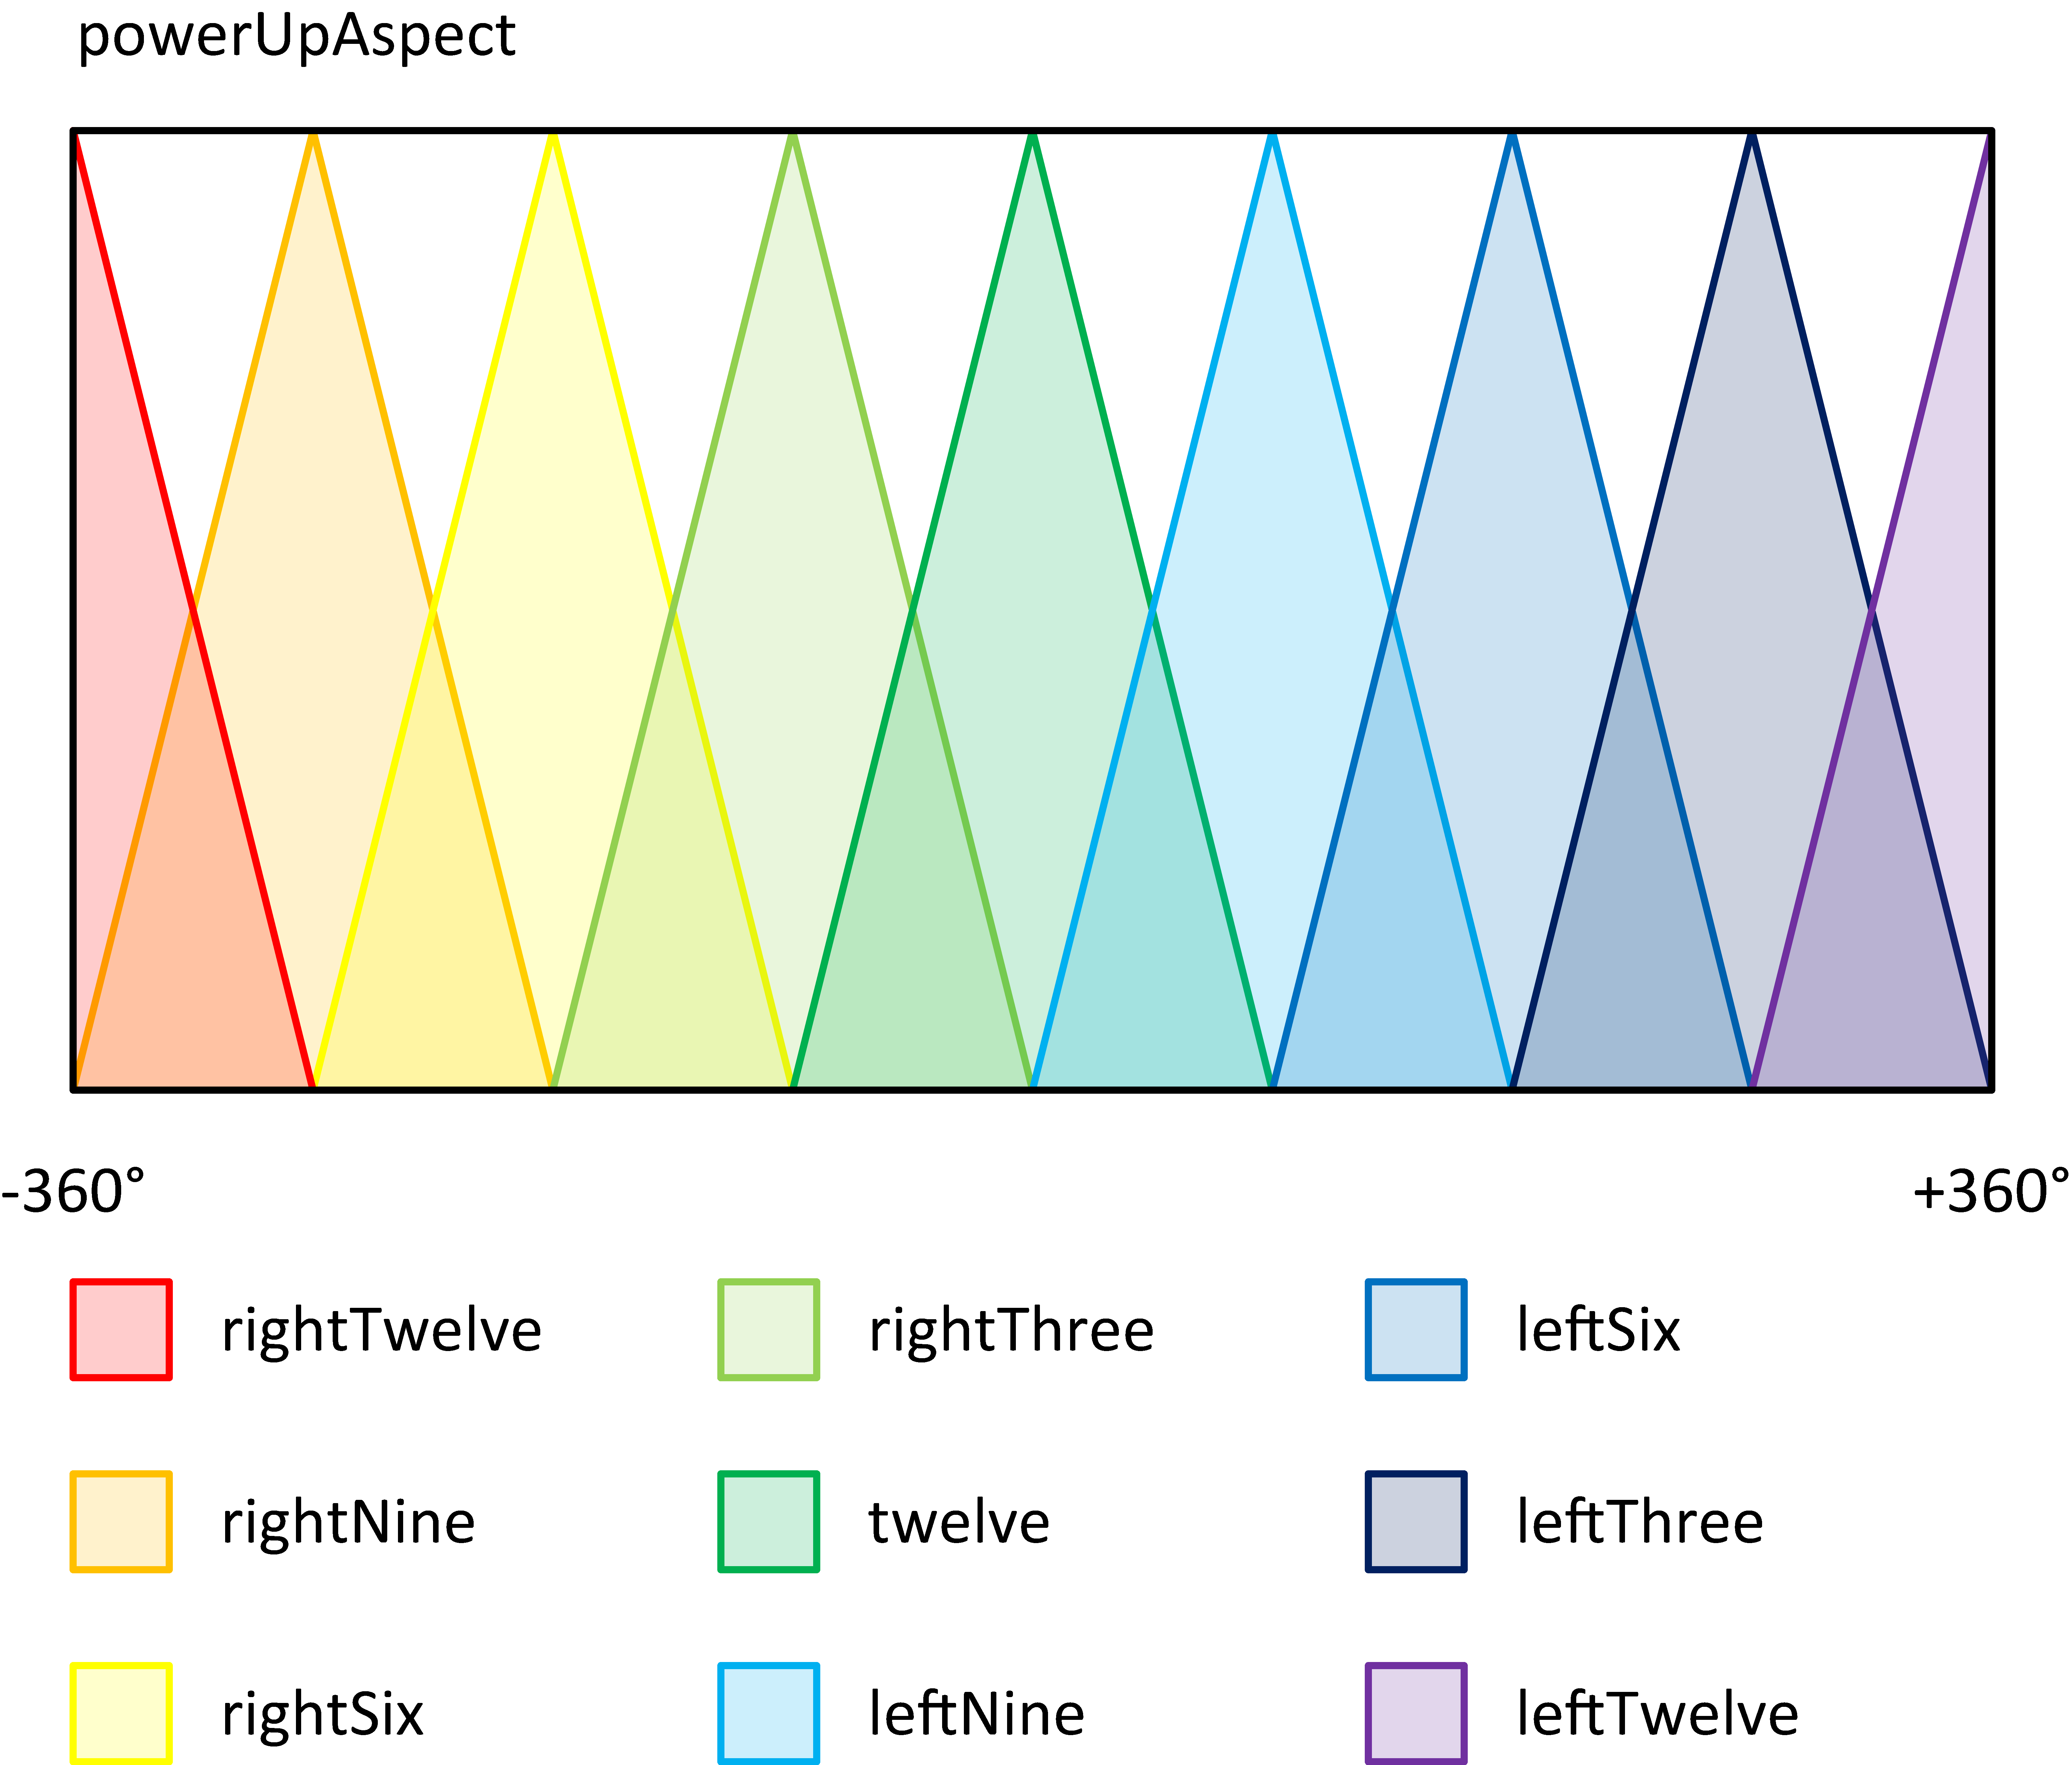
\includegraphics[scale=0.08]{./img/pdf/powerUpAspectSets.pdf}
\end{figure}

\section{Output linguistic variables}

Due to the fact that the fuzzy logic API does not provide a method to prioritize rules, defensive and offensive versions of some output linguistic variables have been defined. Boolean variables are defined, which are then tested to determine which version of the rule is fired, during a given situation.

For example, the defensive turn rule only considers the blast linguistic variables as input, whereas the offensive turn rule considers both target and blast linguistic variables.

\subsection{Defensive rules}

\subsubsection{defensiveTurn}

The \emph{defensiveTurn} linguistic variable defines which heading the saucer will take, in degrees, according to the rules that govern defensive turning. The linguistic variables used as input for \emph{defensiveTurn} are: \mintinline{console}{layerVar = blastDist}, \\ \mintinline{console}{rowVar = blastAngleOff}, and \mintinline{console}{colVar = blastAspect}, creating a 3D rule matrix. Note that \emph{r} and \emph{l} represent right and left in the table.
\\
\\
For example: IF (close) AND (rightSix) AND (zero) THEN (-90) \\
In other words, IF the energy blast is close, AND it is behind the player, AND it's heading towards the player, THEN turn right for 90$^{\circ}$.

\begin{table}[H]
\centering
\caption{\emph{defensiveTurn} \emph{blastDist close}}
\label{Turn rule table}
\begin{tabular}{r|r|r|r|r|r|r|r|r|r}
 		& rTwelve 	& rNine 	& rSix 		& rThree 		& twelve 	& lNine 	& lSix 		& lThree	& lTwelve		\\ \hline
rZero	& 0			& 0			& -90		& 0 		 	& 0			& 0			& -90	 	& 0			& 0				\\
r270	& -90		& 0			& -90		& +180			& +90		& 0			& -90		& +180		& +90			\\
rMerge	& 0			& 0			& -90	 	& 0				& 0			& 0			& -90		& 0			& 0				\\
r90		& -90		& -180		& -90 		& 0				& -90		& -180		& -90		& 0			& +90			\\
zero 	& 0			& 0 		& -90 		& 0				& 0			& 0			& -90		& 0			& 0				\\
l90 	& -90		& 0 		& -90		& +180			& +90		& 0			& -90		& +180		& +90			\\
lMerge	& 0			& 0 		& -90 		& 0				& 0			& 0			& -90		& 0			& 0				\\
l270 	& -90		& -180 		& -90		& 0				& -90		& -180		& -90		& 0			& +90			\\
lZero 	& 0			& 0 		& -90	 	& 0				& 0			& 0  		& -90		& 0			& 0				
\end{tabular}
\end{table}

\begin{table}[H]
\centering
\caption{\emph{defensiveTurn} \emph{blastDist far}}
\label{Turn rule table}
\begin{tabular}{r|r|r|r|r|r|r|r|r|r}
 		& rTwelve 	& rNine 	& rSix 		& rThree 	& twelve 	& lNine 	& lSix 		& lThree	& lTwelve	\\ \hline
rZero	& -180		& 0			& -90		& 0 	 	& 0			& 0			& +90		& 0			& +180		\\
r270	& 0			& 0			& 0			& 0			& 0			& 0			& 0			& 0			& 0			\\
rMerge	& 0			& 0			& 0	 		& 0			& 0			& 0			& 0			& 0			& 0			\\
r90		& 0			& 0			& 0 		& 0			& 0			& 0			& 0			& 0			& 0			\\
zero 	& -180		& 0 		& -90 		& 0			& 0			& 0			& +90		& 0			& +180		\\
l90 	& 0			& 0 		& 0			& 0			& 0			& 0			& 0			& 0			& 0			\\
lMerge	& 0			& 0 		& 0	 		& 0			& 0			& 0			& 0			& 0			& 0			\\
l270 	& 0			& 0	 		& 0 		& 0			& 0			& 0			& 0			& 0			& 0			\\
lZero 	& -180		& 0 		& -90 		& 0			& 0			& 0  		& +90		& 0			& +180		
\end{tabular}
\end{table}

\subsubsection{defensiveSpeed}

The \emph{defensiveSpeed} linguistic variable defines how fast the saucer will travel, according to the rules that govern defensive speed. The linguistic variables used for input for \emph{defensiveSpeed} are: \mintinline{console}{layerVar = blastDist}, \mintinline{console}{rowVar = blastAngleOff}, and \mintinline{console}{colVar = blastAspect}, creating a 3D rule matrix.
\\
\\
For example: IF (close) AND (rightSix) AND (zero) THEN (125) \\
In other words, IF the energy blast is close, AND it is behind the player, AND it's heading towards the player, THEN speed is 125.

\begin{table}[H]
\centering
\caption{\emph{defensiveSpeed} \emph{blastDist close}}
\label{Turn rule table}
\begin{tabular}{r|r|r|r|r|r|r|r|r|r}
 		& rTwelve 	& rNine 	& rSix 		& rThree 		& twelve 	& lNine 	& lSix 		& lThree	& lTwelve		\\ \hline
rZero	& 50		& 125		& 125		& 125 		 	& 50		& 125		& 125 		& 125		& 50			\\
r270	& 50		& 125		& 50		& 125			& 50		& 125		& 50		& 125		& 50			\\
rMerge	& 50		& 125		& 50	 	& 125			& 125		& 125		& 50		& 125		& 50			\\
r90		& 50		& 125		& 50 		& 125			& 125		& 125		& 50		& 125		& 50			\\
zero 	& 50		& 125 		& 125 		& 125			& 50		& 125		& 125		& 125		& 50			\\
l90 	& 50		& 125 		& 50		& 125			& 125		& 125		& 50		& 125		& 50			\\
lMerge	& 50		& 125 		& 50	 	& 125			& 125		& 125		& 50		& 125		& 50			\\
l270 	& 50		& 125	 	& 50 		& 125			& 50		& 125		& 50		& 125		& 50			\\
lZero 	& 50		& 125 		& 125	 	& 125			& 50		& 125  		& 125		& 125		& 50			
\end{tabular}
\end{table}

\begin{table}[H]
\centering
\caption{\emph{defensiveSpeed} \emph{blastDist far}}
\label{Turn rule table}
\begin{tabular}{r|r|r|r|r|r|r|r|r|r}
 		& rTwelve 	& rNine 	& rSix 		& rThree 		& twelve 	& lNine 	& lSix 		& lThree	& lTwelve		\\ \hline
rZero	& 50		& 50		& 75		& 50 		 	& 50		& 50		& 75 		& 50		& 50			\\
r270	& 50		& 50		& 50		& 75			& 50		& 50		& 50		& 75		& 50			\\
rMerge	& 50		& 50		& 50	 	& 50			& 75		& 50		& 50		& 50		& 50			\\
r90		& 50		& 75		& 50 		& 50			& 75		& 75		& 50		& 50		& 50			\\
zero 	& 50		& 50 		& 75 		& 50			& 50		& 50		& 75		& 50		& 50			\\
l90 	& 50		& 50 		& 50		& 75			& 75		& 50		& 50		& 75		& 50			\\
lMerge	& 50		& 50 		& 50	 	& 50			& 75		& 50		& 50		& 50		& 50			\\
l270 	& 50		& 75	 	& 50 		& 50			& 50		& 75		& 50		& 50		& 50			\\
lZero 	& 50		& 50 		& 75	 	& 50			& 50		& 50  		& 75		& 50		& 50			
\end{tabular}
\end{table}

\noindent
Singleton rules have also been added to \emph{defensiveSpeed}, using \emph{powerUpDist} as input:

\begin{itemize}
\item IF (powerUpDist IS far) THEN (defensiveSpeed IS 50)
\item IF (powerUpDist IS near) THEN (defensiveSpeed IS 125)
\item IF (powerUpDist IS close) THEN (defensiveSpeed IS 125)
\end{itemize}

\subsection{Offensive rules}

\subsubsection{offensiveTurn}

The \emph{offensiveTurn} linguistic variable defines which heading the saucer will take, in degrees, according to the rules that govern defensive turning. Two sets of linguistic variables are combined, target variables and blast variables, creating two 3D rule matrices. 

The target linguistic variables used as input for \emph{offensiveTurn} are: \\ \mintinline{console}{layerVar = targetDist}, \mintinline{console}{rowVar = targetEnergyDiff}, and \\ \mintinline{console}{colVar = targetAspect}, creating the 3D rule matrix below.
\begin{table}[H]
\centering
\caption{\emph{offensiveTurn} \emph{targetDist close}}
\label{Turn rule table}
\begin{tabular}{r|r|r|r|r|r|r|r|r|r}
 		& rTwelve 	& rNine 	& rSix 		& rThree 		& twelve 	& lNine 	& lSix 		& lThree	& lTwelve		\\ \hline
losing	& +180		& -90		& 0			& +90 		 	& -180		& -90		& 0 		& +90		& -180			\\
winning	& 0			& +90		& -180		& -90			& 0			& +90		& +180		& -90		& 0			
\end{tabular}
\end{table}

\begin{table}[H]
\centering
\caption{\emph{offensiveTurn} \emph{targetDist near}}
\label{Turn rule table}
\begin{tabular}{r|r|r|r|r|r|r|r|r|r}
 		& rTwelve 	& rNine 	& rSix 		& rThree 		& twelve 	& lNine 	& lSix 		& lThree	& lTwelve		\\ \hline
losing	& +180		& 0			& 0			& 0 		 	& -180		& 0			& 0 		& 0			& -180			\\
winning	& 0			& +90		& -180		& -90			& 0			& +90		& +180		& -90		& 0			
\end{tabular}
\end{table}

The blast linguistic variables used as input for \emph{offensiveTurn} are: \\ \mintinline{console}{layerVar = blastDist}, \mintinline{console}{colVar = blastAngleOff}, and \mintinline{console}{rowVar = blastAspect}, creating another 3D rule matrix.

\begin{table}[H]
\centering
\caption{\emph{offensiveTurn} \emph{blastDist close}}
\label{Turn rule table}
\begin{tabular}{r|r|r|r|r|r|r|r|r|r}
 		& rTwelve 	& rNine 	& rSix 		& rThree 		& twelve 	& lNine 	& lSix 		& lThree	& lTwelve		\\ \hline
rZero	& 0			& 0			& -90		& 0 		 	& 0			& 0			& -90	 	& 0			& 0				\\
r270	& -90		& 0			& -90		& +180			& +90		& 0			& -90		& +180		& +90			\\
rMerge	& 0			& 0			& -90	 	& 0				& 0			& 0			& -90		& 0			& 0				\\
r90		& -90		& -180		& -90 		& 0				& -90		& -180		& -90		& 0			& +90			\\
zero 	& 0			& 0 		& -90 		& 0				& 0			& 0			& -90		& 0			& 0				\\
l90 	& -90		& 0 		& -90		& +180			& +90		& 0			& -90		& +180		& +90			\\
lMerge	& 0			& 0 		& -90 		& 0				& 0			& 0			& -90		& 0			& 0				\\
l270 	& -90		& -180 		& -90		& 0				& -90		& -180		& -90		& 0			& +90			\\
lZero 	& 0			& 0 		& -90	 	& 0				& 0			& 0  		& -90		& 0			& 0				
\end{tabular}
\end{table}

\begin{table}[H]
\centering
\caption{\emph{offensiveTurn} \emph{blastDist far}}
\label{Turn rule table}
\begin{tabular}{r|r|r|r|r|r|r|r|r|r}
 		& rTwelve 	& rNine 	& rSix 		& rThree 	& twelve 	& lNine 	& lSix 		& lThree	& lTwelve	\\ \hline
rZero	& -180		& 0			& -90		& 0 	 	& 0			& 0			& +90		& 0			& +180		\\
r270	& 0			& 0			& 0			& 0			& 0			& 0			& 0			& 0			& 0			\\
rMerge	& 0			& 0			& 0	 		& 0			& 0			& 0			& 0			& 0			& 0			\\
r90		& 0			& 0			& 0 		& 0			& 0			& 0			& 0			& 0			& 0			\\
zero 	& -180		& 0 		& -90 		& 0			& 0			& 0			& +90		& 0			& +180		\\
l90 	& 0			& 0 		& 0			& 0			& 0			& 0			& 0			& 0			& 0			\\
lMerge	& 0			& 0 		& 0	 		& 0			& 0			& 0			& 0			& 0			& 0			\\
l270 	& 0			& 0	 		& 0 		& 0			& 0			& 0			& 0			& 0			& 0			\\
lZero 	& -180		& 0 		& -90 		& 0			& 0			& 0  		& +90		& 0			& +180		
\end{tabular}
\end{table}

\subsubsection{offensiveSpeed}

The \emph{offensiveSpeed} linguistic variable defines how fast the saucer will travel, according to the rules that govern offensive speed. Two sets of linguistic variables are used as input, target variables and blast variables.

The target linguistic variables used as input for \emph{offensiveSpeed} are: \\ \mintinline{console}{rowVar = targetDist}, and \mintinline{console}{colVar = targetEnergyDiff}

\begin{table}[H]
\centering
\caption{\emph{offensiveSpeed} target variables}
\label{Turn rule table}
\begin{tabular}{r|r|r}
 		& losing 	& winning	\\ \hline
close	& 125		& 50		\\
near	& 75		& 75		\\
far		& 50		& 125			
\end{tabular}
\end{table}

The blast linguistic variables used as input for \emph{offensiveSpeed} are: \\ \mintinline{console}{layerVar = blastDist}, \mintinline{console}{colVar = blastAngleOff}, and \mintinline{console}{rowVar = blastAspect}

\begin{table}[H]
\centering
\caption{\emph{offensiveSpeed} \emph{blastDist close}}
\label{Turn rule table}
\begin{tabular}{r|r|r|r|r|r|r|r|r|r}
 		& rTwelve 	& rNine 	& rSix 		& rThree 		& twelve 	& lNine 	& lSix 		& lThree	& lTwelve		\\ \hline
rZero	& 50		& 50		& 125		& 50 		 	& 50		& 50		& 125 		& 50		& 50			\\
r270	& 50		& 50		& 50		& 125			& 50		& 50		& 50		& 125		& 50			\\
rMerge	& 50		& 50		& 50	 	& 50			& 125		& 50		& 50		& 50		& 50			\\
r90		& 50		& 125		& 50 		& 50			& 125		& 125		& 50		& 50		& 50			\\
zero 	& 50		& 50 		& 125 		& 50			& 50		& 50		& 125		& 50		& 50			\\
l90 	& 50		& 50 		& 50		& 125			& 125		& 50		& 50		& 125		& 50			\\
lMerge	& 50		& 50 		& 50	 	& 50			& 125		& 50		& 50		& 50		& 50			\\
l270 	& 50		& 125	 	& 50 		& 50			& 50		& 125		& 50		& 50		& 50			\\
lZero 	& 50		& 50 		& 125	 	& 50			& 50		& 50  		& 125		& 50		& 50			
\end{tabular}
\end{table}

\begin{table}[H]
\centering
\caption{\emph{offensiveSpeed} \emph{blastDist far}}
\label{Turn rule table}
\begin{tabular}{r|r|r|r|r|r|r|r|r|r}
 		& rTwelve 	& rNine 	& rSix 		& rThree 		& twelve 	& lNine 	& lSix 		& lThree	& lTwelve		\\ \hline
rZero	& 50		& 50		& 75		& 50 		 	& 50		& 50		& 75 		& 50		& 50			\\
r270	& 50		& 50		& 50		& 75			& 50		& 50		& 50		& 75		& 50			\\
rMerge	& 50		& 50		& 50	 	& 50			& 75		& 50		& 50		& 50		& 50			\\
r90		& 50		& 75		& 50 		& 50			& 75		& 75		& 50		& 50		& 50			\\
zero 	& 50		& 50 		& 75 		& 50			& 50		& 50		& 75		& 50		& 50			\\
l90 	& 50		& 50 		& 50		& 75			& 75		& 50		& 50		& 75		& 50			\\
lMerge	& 50		& 50 		& 50	 	& 50			& 75		& 50		& 50		& 50		& 50			\\
l270 	& 50		& 75	 	& 50 		& 50			& 50		& 75		& 50		& 50		& 50			\\
lZero 	& 50		& 50 		& 75	 	& 50			& 50		& 50  		& 75		& 50		& 50			
\end{tabular}
\end{table}

\subsection{Overrides}

The following output linguistic variables do not have offensive or defensive versions, but are controlled by testing boolean variables which determine when to fire these rules. For example, \emph{firepower}'s rate of fire is controlled by a boolean variable, which becomes \mintinline{console}{true} when there are only a certain number of enemies left in the battle space.

\subsubsection{firepower}

The \emph{firepower} linguistic variable defines how much energy to commit to firing the cannon, according to the rules that govern firepower. \emph{targetDist} is used as input. Additionally, the number of remaining enemy saucers and whether or not there is a nearby powerup determines the rate of fire, and the implementation of decision making will be shown as Java code.

The strategy is to be conservative with firepower unless there is a powerup nearby. If so, increase to maximum rate of fire to deter any enemy saucers that may be near the powerup from retrieving it, while the player moves directly to the powerup. If there are only two enemies left, increase rate of fire to medium, and if there is one enemy left, increase rate of fire to maximum. The strategy is to become more aggressive towards the end of the battle, since the result could be a tie if other saucers remain at the end of the battle.
\\
\\
The \emph{firepower} rules relating to \emph{targetDist} are:

\begin{itemize}
\item IF (targetDist IS far) THEN (firepower IS 0)
\item IF (targetDist IS near) THEN (firepower IS 100)
\item IF (targetDist IS close) THEN (firepower IS 100)
\end{itemize}

\noindent
The following variables determine the rate of fire:

\begin{listing}[H]
\caption{\emph{firepower} variables}
\begin{javacode}
private static final double DEFENCE_ROF = 0.01;
private static final double OFFENCE_ROF = 0.05;
private static boolean isLastTwoTargets; // true when only two enemy saucers remain
private static boolean isLastTarget; // true when only one enemy saucer remains
private static boolean isPowerUpNear; // true when powerup within 1200.575m
\end{javacode}
\end{listing}

\noindent
Rate of fire is controlled by the \mintinline{console}{getFirePower()} method:

\begin{listing}[H]
\caption{\mintinline{console}{getFirePower()}}
\begin{javacode}
public double getFirePower() throws Exception {

    // max rate of fire
    if(isLastTarget || isPowerUpNear) {
        return firePower.getValue();
    // medium rate of fire
    } else if(isLastTwoTargets) {
        if(Math.random() < OFFENCE_ROF) {
            return firePower.getValue();
        } else {
            return 0.0;
        }
    // min rate of fire
    } else {
        if(Math.random() < DEFENCE_ROF) {
            return firePower.getValue();
        } else {
            return 0.0;
        }
    }
}
\end{javacode}
\end{listing}

\subsubsection{getPowerUpTurn}

The \emph{getPowerUpTurn} linguistic variable defines which heading the saucer will take, in degrees, according to the rules that govern turning towards a nearby powerup. This linguistic variable is used to override the player's current turning regime, and ensure that it heads straight for a powerup without dodging any energy blasts. This rule is fired in conjunction with an increased rate of fire, as well as deploying the shield to protect itself as it attempts to retrieve a powerup.

\emph{powerUpDist} and \emph{powerUpAspect} are used as inputs, as well as a boolean variable which determines when this rule overrides all other turn rules.

\begin{table}[H]
\centering
\caption{\emph{getPowerUpTurn}}
\label{Turn rule table}
\begin{tabular}{r|r|r|r}
 		& close 	& near	 	& far 		\\ \hline
rTwelve	& 0			& 0			& 0			\\
rNine	& +90		& +90		& 0			\\
rSix	& -180		& -180		& 0		 	\\
rThree	& -90		& -90		& 0	 		\\
twelve 	& 0			& 0 		& 0 		\\
lNine 	& +90		& +90 		& 0			\\
lSix	& +180		& +180 		& 0 		\\
lThree 	& -90		& -90 		& 0			\\
lTwelve	& 0			& 0 		& 0	 	
\end{tabular}
\end{table}

\noindent
The boolean variable determines when \emph{getPowerUpTurn} overrides other turn rules:

\begin{listing}[H]
\caption{\emph{getPowerUpTurn} variable}
\begin{javacode}
private static boolean isPowerUpNear; // true when powerup within 1200.575m
\end{javacode}
\end{listing}

\noindent
\emph{getPowerUpTurn} overrides other turn rules in the \mintinline{console}{getTurn()} method:

\begin{listing}[H]
\caption{\mintinline{console}{getTurn()}}
\begin{javacode}
public double getTurn() throws Exception {

    // override turn rules if powerup is nearby
    if(isPowerUpNear) {
        return getPowerUpTurn.getValue();
    }
	
    // use offensiveTurn if last two, or last target
    if(isLastTarget || isLastTwoTargets) {
        return offensiveTurn.getValue();
    } else {
        return defensiveTurn.getValue();
    }
}
\end{javacode}
\end{listing}

\subsubsection{shield}

The \emph{shield} linguistic variable defines when to deploy the shield, according to the rules that govern shield deployment. The universe of disclosure is between 0 and 1. This linguistic variable uses powerup, blast and \emph{myEnergy} variables as input, and uses the following sets: \mintinline{console}{layerVar = powerUpDist}, \mintinline{console}{rowVar = myEnergy}, and \mintinline{console}{colVar = blastDist}, creating a 3D rule matrix. 

\begin{table}[H]
\centering
\caption{\emph{shield} \emph{powerUpDist close}}
\label{Turn rule table}
\begin{tabular}{r|r|r}
 			& close 	& far	 	\\ \hline
lowEnergy	& 1			& 0			\\
highEnergy	& 1			& 0		
\end{tabular}
\end{table}

\begin{table}[H]
\centering
\caption{\emph{shield} \emph{powerUpDist near}}
\label{Turn rule table}
\begin{tabular}{r|r|r}
 			& close 	& far	 	\\ \hline
lowEnergy	& 0			& 0			\\
highEnergy	& 1			& 0		
\end{tabular}
\end{table}

\begin{table}[H]
\centering
\caption{\emph{shield} \emph{powerUpDist near}}
\label{Turn rule table}
\begin{tabular}{r|r|r}
 			& close 	& far	 	\\ \hline
lowEnergy	& 0			& 0			\\
highEnergy	& 0			& 0		
\end{tabular}
\end{table}

\noindent
Boolean variable \mintinline{console}{isPowerUpNear} is tested to determine when to deploy the shield, and the crisp output is converted to a boolean value in \mintinline{console}{getShields()} in order to function:

\begin{listing}[H]
\caption{\mintinline{console}{getShields()}}
\begin{javacode}
public boolean getShields() throws Exception {

    // only deploy shield if powerup is nearby
    if(isPowerUpNear) {
        // convert output to boolean
        return shield.getValue() > 0.5;
    } else {
        return false;
    }
}
\end{javacode}
\end{listing}